\documentclass[11pt,a4paper,twoside]{report}

%--------------------------------------------------
% global definitions to be used in the front page
%--------------------------------------------------
\providecommand{\coursename}{Design and Implementation of Mobile Applications}
\providecommand{\documentsubtitle}{Documentation}
\providecommand{\annoacc}{2013-2014}
\providecommand{\principaladvisor}{Prof. Luciano Baresi}
\providecommand{\firstauthor}{Claudio Rizzo}
\providecommand{\firstauthorid}{800471}
\providecommand{\secondauthor}{Emanuele Uliana}
\providecommand{\secondauthorid}{799256}

\title{Watch Dog}
\author{\firstauthor, \secondauthor}

\usepackage[margin=3cm]{geometry} % margins set here are for the TITLE page...


\usepackage[utf8]{inputenc}
\usepackage[english]{babel}
\usepackage{tikz}
\usetikzlibrary{arrows,positioning, decorations.text}

\usepackage{graphicx}
\usepackage{booktabs}
\usepackage{listings}

\lstset{columns=fullflexible}

\usepackage[T1]{fontenc}
\usepackage{palatino}
\usepackage{mathpazo} 
\lstset{basicstyle=\ttfamily}

\usepackage[pdfauthor={\firstauthor, \secondauthor}, pdftitle={WatchDog - Design Document}, colorlinks, linkcolor=black, urlcolor=black]{hyperref}

\usepackage{amsmath}
\usepackage{amsthm}
\newtheoremstyle{note} % name
	{\topsep} 	% Space above
	{\topsep} 	% Space below
	{\small}		% Body font
	{}		% Indent amount
	{\small\bfseries}% Theorem head font
	{:}		% Punctuation after theorem head
	{.5em}	% Space after theorem head
	{}		% Theorem head spec (can be left empty, meaning ‘normal’)
\theoremstyle{note}
\newtheorem*{nota}{Nota}	
%
\usepackage{settings/frontesp}




\usepackage{fancyhdr}
%% Cambia il carattere delle didascalie delle figure %%
\usepackage[font=small,format=plain,labelfont=bf,up,textfont=it,up]{caption}


%per le tabelle lunghe e particolari
\usepackage{lscape}

\setlength{\parindent}{0in}  %%solo una proposta: così non serve
% più il \noindent dopo \\

%% Alloy code begins
\usepackage{color}
\usepackage{xcolor}
\usepackage[normalem]{ulem}
\usepackage{caption}
\DeclareCaptionFont{white}{\color{white}}



%%%%% 

%e.g.
%\begin{lstlisting}[label=some-code,caption=Some Code]
%public void here() {
%	goes().the().code()
%}
%\end{lstlisting}



%Alloy code ends





\begin{document}


\titlep
\newgeometry{top=4cm,bottom=4cm,right=4cm,left=4cm}
%% STILE DELLE INTESTAZIONI %%

\pagestyle{fancy}
\renewcommand{\chaptermark}[1]{\markboth{#1}{}} % aggiungi \thechapter.\ per anche il numero capitolo
%\renewcommand{\sectionmark}[1]{\markright{#1}} % titoli di sezione
\fancyhf{}
\fancyhead[RE,RO]{\small\thepage}
\fancyhead[LE,LO]{\small\em\leftmark} % \leftmark = 2.TitoloCapitolo, \rightmark = TitoloSezione
%\fancyhead[LO]{\small\em\rightmark}  % LO = Left Odd, RO = Right Odd, LE = Left Even, RE = Right Even
\fancypagestyle{plain}{ % titolo di sezione e simili
	\fancyhf{} % remove everything
	\renewcommand{\headrulewidth}{0pt} % remove lines as well
	\renewcommand{\footrulewidth}{0pt}
}

%%% Cambia il carattere dei titoli di sezione %%
%\usepackage{titlesec}
%\titleformat{\section}{\Large\bfseries\sffamily}{\thesection}{1em}{}

%% Stile dei titoli di capitolo %%
\makeatletter
\def\thickhrulefill{\leavevmode \leaders \hrule height 0.7ex \hfill \kern \z@}
\def\@makechapterhead#1{%
  \vspace*{10\p@}%
  {\parindent \z@ \centering \reset@font
        %\thickhrulefill
        \par\nobreak \vspace{3\p@}
        {\huge \bfseries \rmfamily \strut \thechapter.\ #1}\par\nobreak
        \interlinepenalty\@M
        \hrule
        \vspace*{10\p@}%
    \vskip 30\p@
  }}

\def\@makeschapterhead#1{%
  \vspace*{10\p@}%
  \vspace*{10\p@}%
  {\parindent \z@ \centering \reset@font
        %\thickhrulefill
        \par\nobreak \vspace{3\p@}
        {\huge \bfseries \rmfamily \strut #1}\par\nobreak
        \interlinepenalty\@M
        \hrule
        \vspace*{10\p@}%
    \vskip 30\p@
  }}

\tableofcontents
\cleardoublepage


% --------------------------------------------------------------------------------------------------------------------
% Capitoli

% \include con i nomi dei capitoli

\chapter{Project context and purpose }
\label{cap:Introduction} 

\section{Context}

Watchdog is an application for Android devices developed by Claudio Rizzo
and Emanuele Uliana for the "Design and Implementation of Mobile Appli-
cations" (DIMA in short) course at "Politecnico di Milano, Corso di studi in
Ingegneria Informatica Magistrale". The advisor is professor Luciano Baresi
from the Deepse (Dependable, Evolvable, Pervasive Software Engineering)
group of the Deib (Dipartimento di Elettronica, Informazione e Bioingegne-
ria).

\section{Purpose}

The application purpose is to provide a way to remote control a mobile phone
from another cellphone: this is very useful in case of theft or loss, since it’s
possible to localize the target phone or to trigger a full volume repeating
alarm sound. The application is mainly intended to be used by the same user
on two (or more) different mobiles, althought it’s not mandatory.



\chapter{Project Planning}
\label{cap:Planning} 

\section{Overview}

We had the idea to develop a remote control application after seeing there
was not something similar not embedded in a more general application (in
fact every anti-malware for mobile devices have a similar functionality, but it
comes along with many others features) and because we really like the se-
curity/privacy (and cryptography) aspects of computer science. We planned
the security/cryptography aspects from the beginning, such that the Confi-
dentiality/Integrity/Availability paradigm is always respected along with the
extremely important authentication and non-repudiation aspects.

\chapter{Requirements Analysis}
\label{cap:RequirementsAnalysis} 


\section{Actors}

As said before, the main actor is usually a single user which uses the ap-
plication on two different mobile phones, one being the stolen/lost one and
the other the rescue one. It’s also possible a second actor to exists: a (very)
trusted friend may be the one who sends remote commands to the target tele-
phone; since a password authentication scheme is employed, it’s not possible
to do any abuse in this case.

\section{Functional Requirements}

The application allows the user do to the following tasks:

\begin{itemize}
 \item Initialization
 \item Mobile Phone Association
 \item Password Change
 \item Unilateral Deassociation
 \item Remote Localization
 \item Mobile Phone Mark
 \item Remote Alarm Triggering
 \item Local Alarm Off
 \item Perimeter Selection
\end{itemize}

\section{Non Functional Requirements}

The remote control of a cellphone is a critical activity and has many security
and privacy requirements: the next paragraphs show them briefly: for in-depth
explainations see the design section (4.3). %metti il riferimento latexiano

\subsection{Privacy and Security: problems and Solutions}

\bfseries 
Sender authentication:
\normalfont
While the sender (telephone) authentication plays indeed a key role, it’s even
more crucial the authentication of the person behind a control message; that’s
the reason for employing a password based authentication scheme: in the
initialization wizard the user is required to insert a password which is going
to be needed to send a message to that telephone (the basic assumption
is the password is known only by the mobile owner and by some people,
possibly no one, he trusts). The password is stored hashed with SHA-256 in
the application preferences, along with the hashing salt (a random token) to
avoid both time-to-memory attacks (such as rainbow tables) and the equality
of two hashes generated from two equal passwords; the salt is sent to another
telephone after the process of public keys authentication (See section 4.3.6).


\bfseries 
Integrity:
\normalfont
The message received must be exactly the one sent: every transmission error
or tampering must be detected and cause the abort of the current command
session: no retransmission is done.


\bfseries
Authentication:
\normalfont
The receiver must have a secure way to understand which telephone the
received message comes from.


\bfseries 
Non forgeability:
\normalfont
Nobody should be able to forge a command message which is both valid and
correctly authenticated.


\bfseries 
Non Repudation:
\normalfont
The sender must not be able to deny he sent a specific message (if he actually
did it).
Digitally signing every command message can ensure integrity, authentica-
tion, non repudiation and a weak defense against non forgeability: symmetric
encryption (and in particular AES-256 in GCM mode of operation) is needed
for full protection.


\bfseries
Message Confidentiality:
\normalfont
No one should be able to detect that and which command is sent to a mobile
phone, so the command message is encrypted with the symmetric cipher
AES-256 in GCM mode of operation (used for performance reasons and for a
supplementary integrity check).



\bfseries
Asymmetric keys management:
\normalfont
Asymmetric keys management
Digital signatures (and shared secrets computation as we will see) require
asymmetric cryptography: in the initialization wizard the application gener-
ates and stores in the preferences a key pair based on the elliptic curves; the
reasons for this choice are performances and the smaller key length with re-
spect to other keys (like RSA and DSA ones) at a fixed level of security. This
makes the 140 characters (bytes) Android limit for a single sms no more a
problem.


\bfseries
Symmetric key/initialization vector management:
\normalfont
AES-256, being a symmetric cipher, encrypts and decrypts a specific message
with the same key, and, given the communication channel is not secure, the
two parts must agree on the same key in some way; in particular ECDH is
used to compute a common secret once and for all, then, when in need to
send a message, the sender picks up a random 32 bytes salt, forwards it to
the receiver, then both parts use a keyschedule algorithm (PBKDF2 with
HMAC-SHA-256) to derive the same key starting from the secret and the
salt. Furthermore the GCM mode of operation requires for every message the
sender to generate a 12 bytes random initialization vector and to send it to
the receiver.


\bfseries
Public keys mutual authentication:
\normalfont

While dealing with asymmetric cryptography, the main problem is to bind a
public key with a real user to avoid active Man-In-The-Middle (MITM from
now on) attacks. Neither a Pulic Key infrastructure (PKI) or a Web Of Trust
(WOT) is employed, because they are both potentially insecure for various
reasons (in the PKI case the presence of a trusted element, a certification
autorithy hierarchy, which may be compromised/untrusted/fake; in the WOT
case the presence of a net of trusted elements, the ones who signed a specific
public key, which might be fake/bad persons; furthermore a key with no
signatures is not automatically a fake one, but there isn’t a way to tell), so
the application uses a modified version of the Socialist Millionaire Protocol
(SMP) to authenticate to each one each other key; this requires the two parts
to have a common secret (an answer to a particular question set up on the fly
by the users during the SMP), which is easy to achieve, since the two users
are likely to be the same person or two people who trust themselves.

\subsection{Performance}

We chose the crypto algorithms with an eye on the performances of the
whole system: the key idea is the bottleneck must be the sms and not the
computation time required by the encryptions/decryptions; for this reason
the command messages are encrypted with a symmetric algorithm and not
with RSA or ElGamal (or another asymmetric algorithm), since symmetric
cryptography is faster than asymmetric at least by two orders of magnitude
(they are very likely to be 3 anyway); however to do ECDH and ECDSA
the application needs also an asymmetric key pair, which is generate during
the intitial wizard once an for all, so an acceptable overhead. The public
keys mutual validation (SMP + ECDH in practice) takes some time, but it’s
done only one time per association, which means two telephones have to do it
only when they associate themselves. Finally the digital signature/verification
process are quite fast and so is the key-derivation from the secret and the
salt.











\chapter{Use Cases}
\label{cap:UseCases} 


\section{Initialization}
The first time the appliction is opened the user sees a welcome message and his
prompted to comlete the initialization wizard which consists in selecting and
confirming a password which will be the one needed by other telephones/users
to send commands to that mobile. The password scheme forces to select an
alphanumeric string (some special characters are also allowed) between 8-
20 characters and with at least a letter and a number. In case of error
(bad password/confirmation password different from the base one) the user is
notified back and asked to retry. In case of success the application redirects
to the main view, which is the "sms localization" one.

\subsection{Activity Diagram}

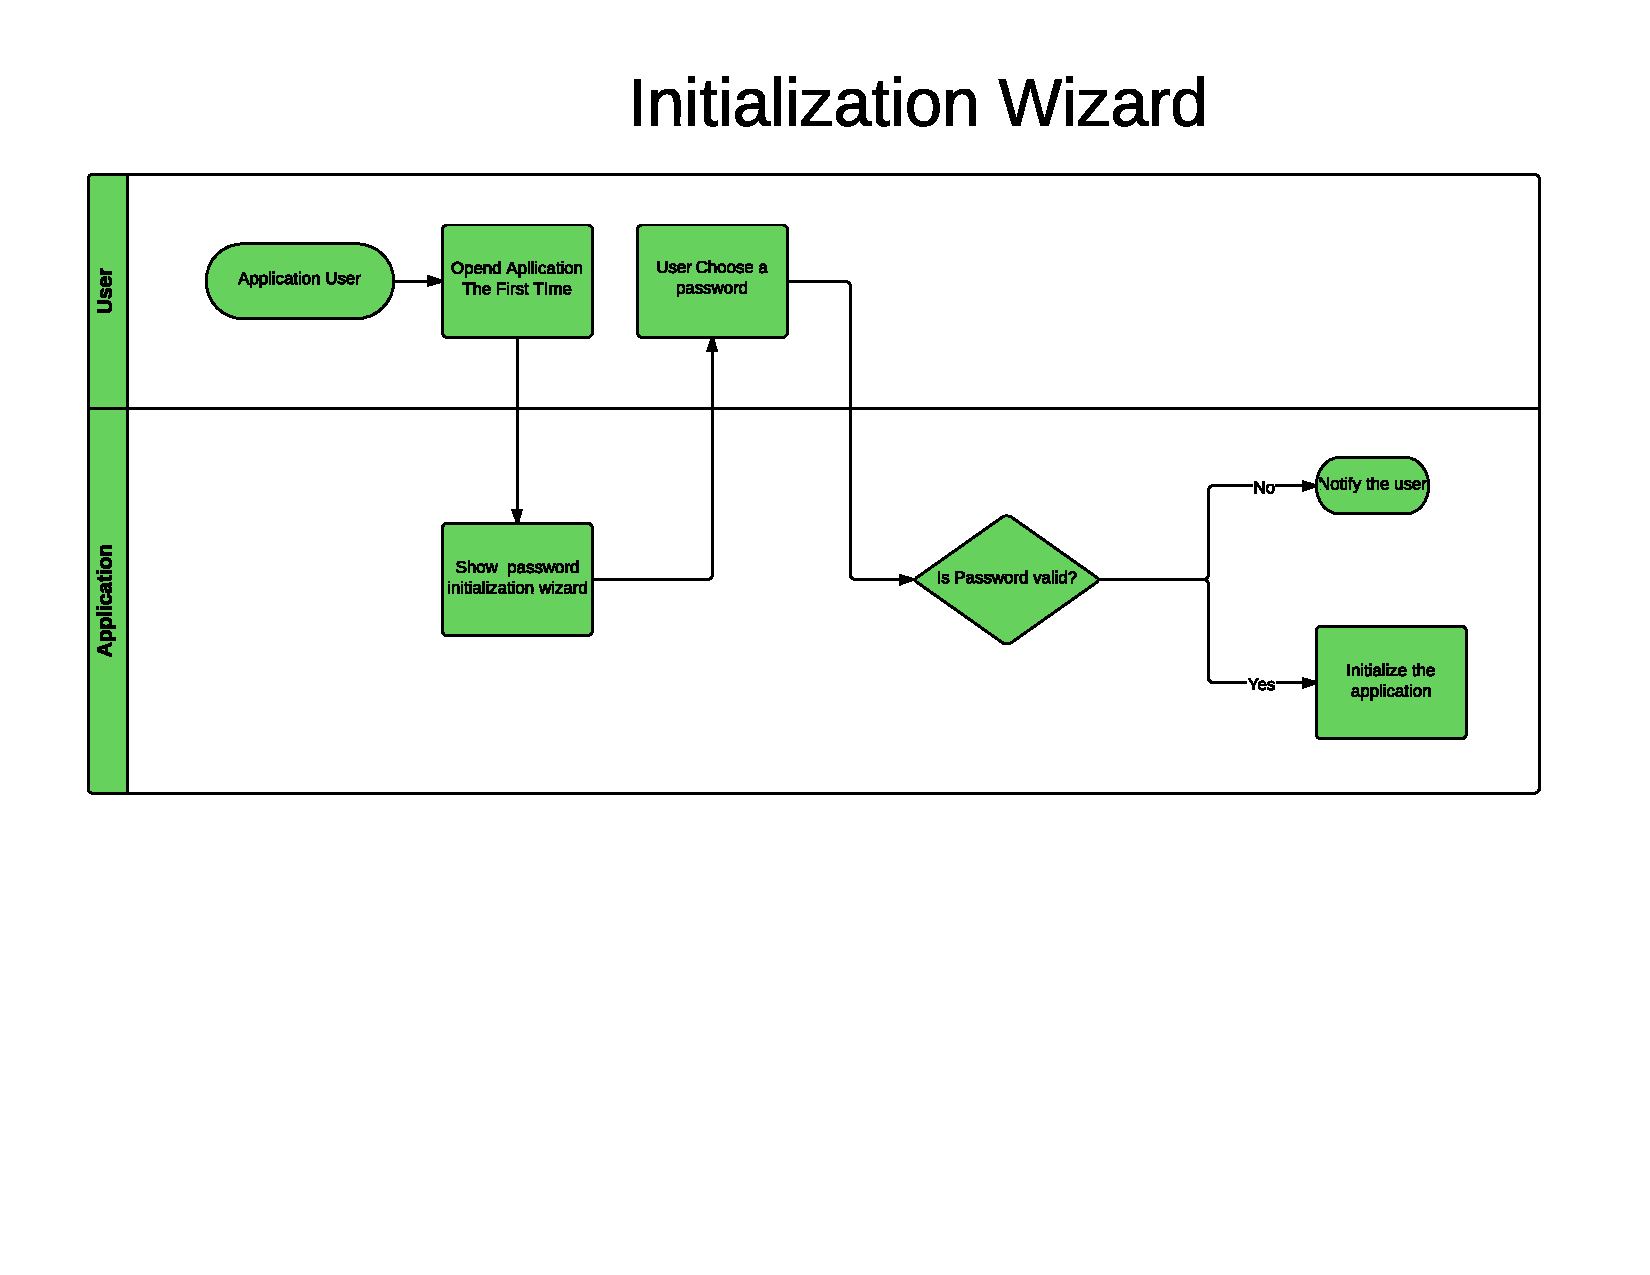
\includegraphics[scale=0.5]{images/initialization_activity}

\newpage
\subsection{User Interface Design}

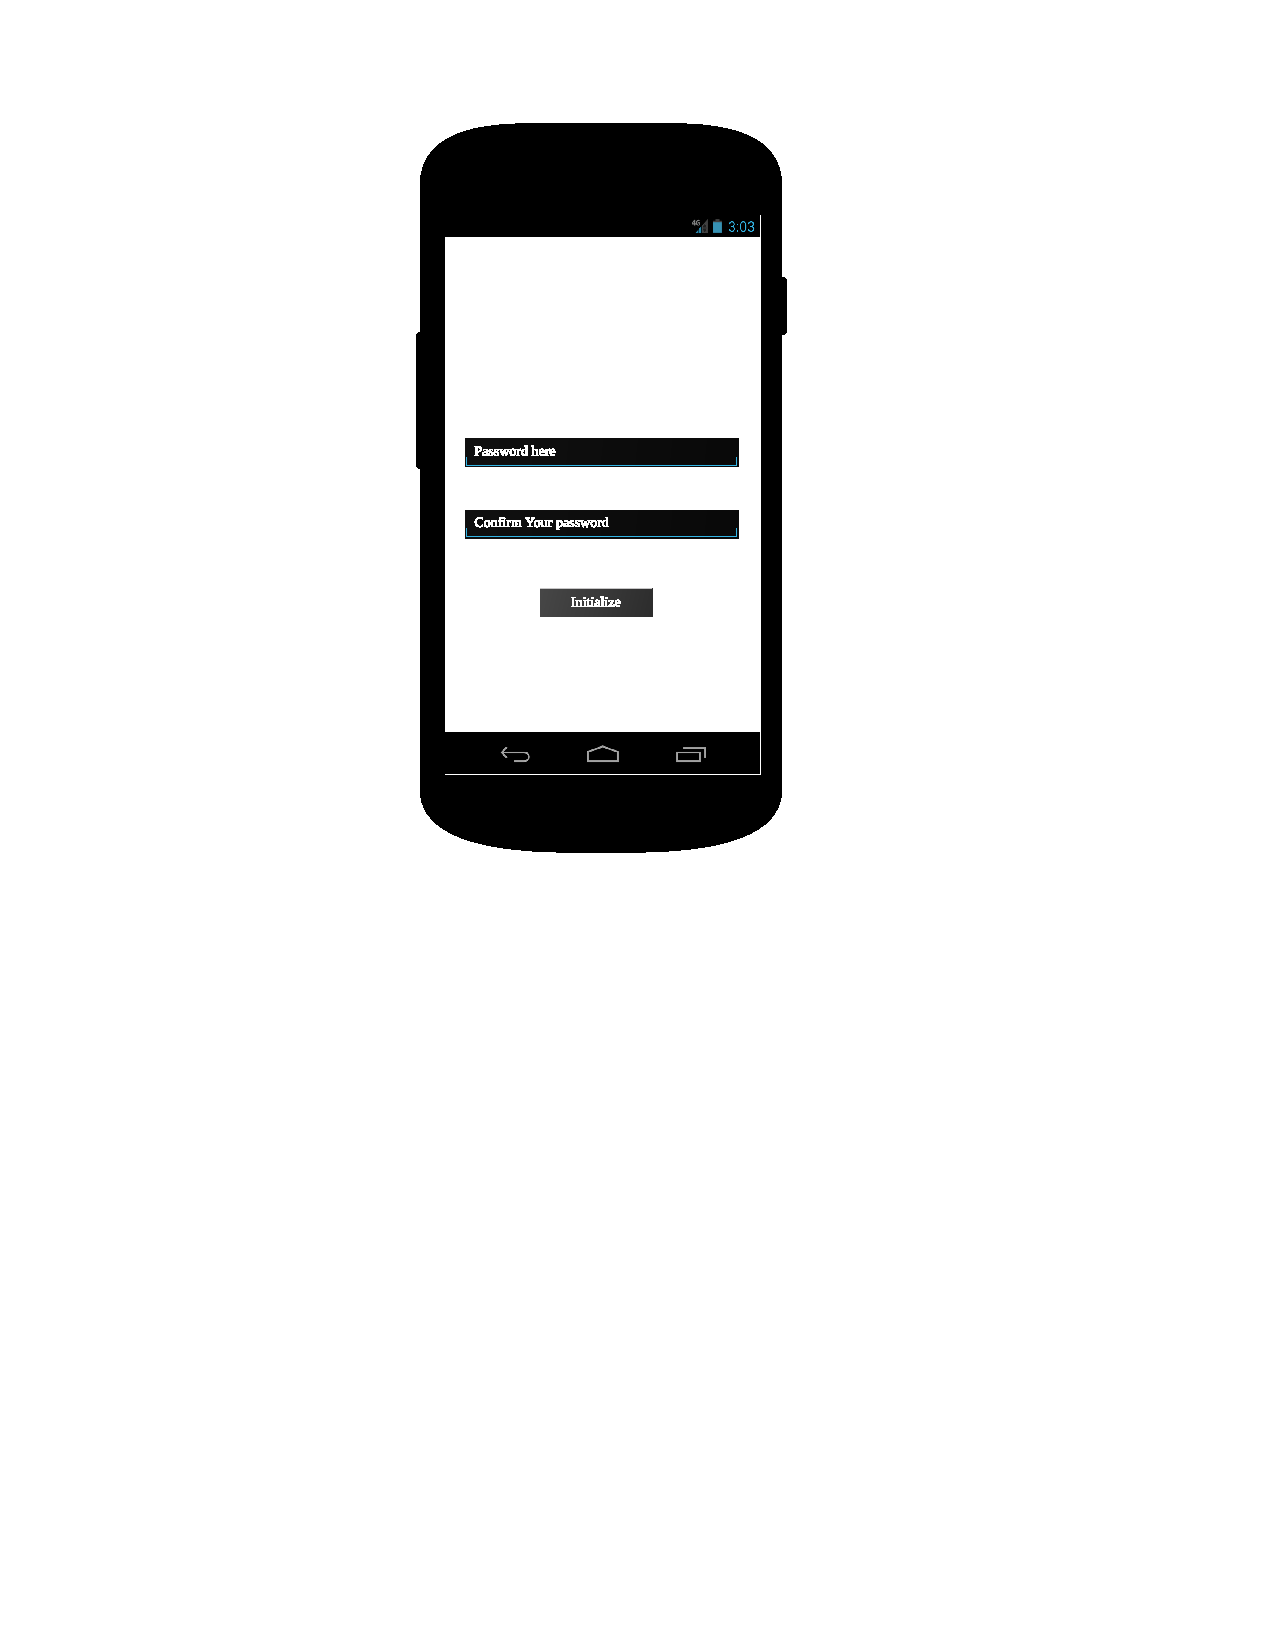
\includegraphics[scale=0.7]{images/initialization_design}


\section{Mobile Phone Association}
For enhanced security it’s required two telephones are associated before they
can send commands to the other one; the association is bidirectional and can
be removed only locally (the other telephone won’t know anything, but will
obviously fail in sending commands). This totally cuts away the possibility of
a Man In The Middle (MITM) both active and passive. A user who wants
to associate his telephone with another one first selects a secret question
and a secret answer and sends the first to the other mobile, whose user can
decide to accept or refuse the request. In the second case the first user is
notified back and the association ends with a "failure", otherwise the second
user types what he thinks is the secret answer and selects his own secret
question/answer. The first user now has to type the answer to that question
and, if all goes smooth, the association is done. Every passage is done by
sms sending.

\newpage
\subsection{Activity Diagram}

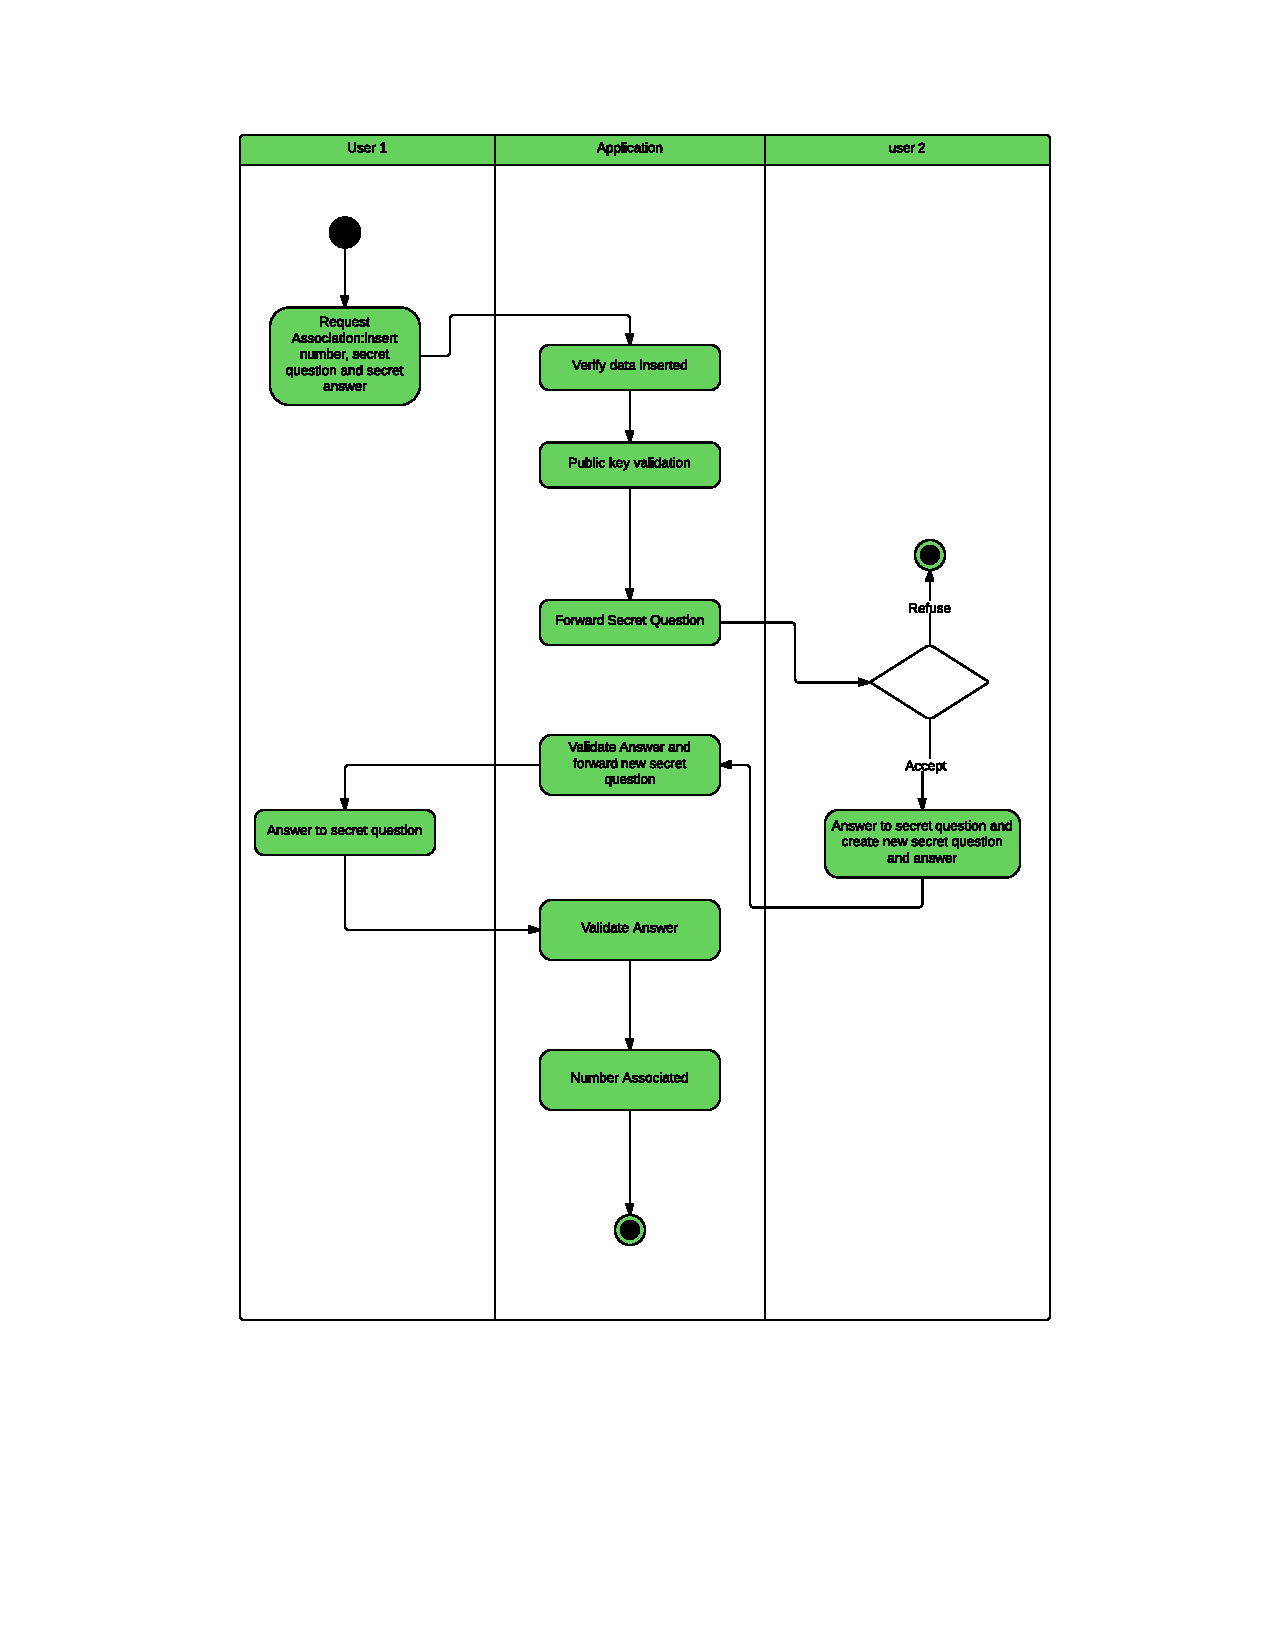
\includegraphics[scale=0.7]{images/SMP_activity}

\newpage
\subsection{User Interface Design}

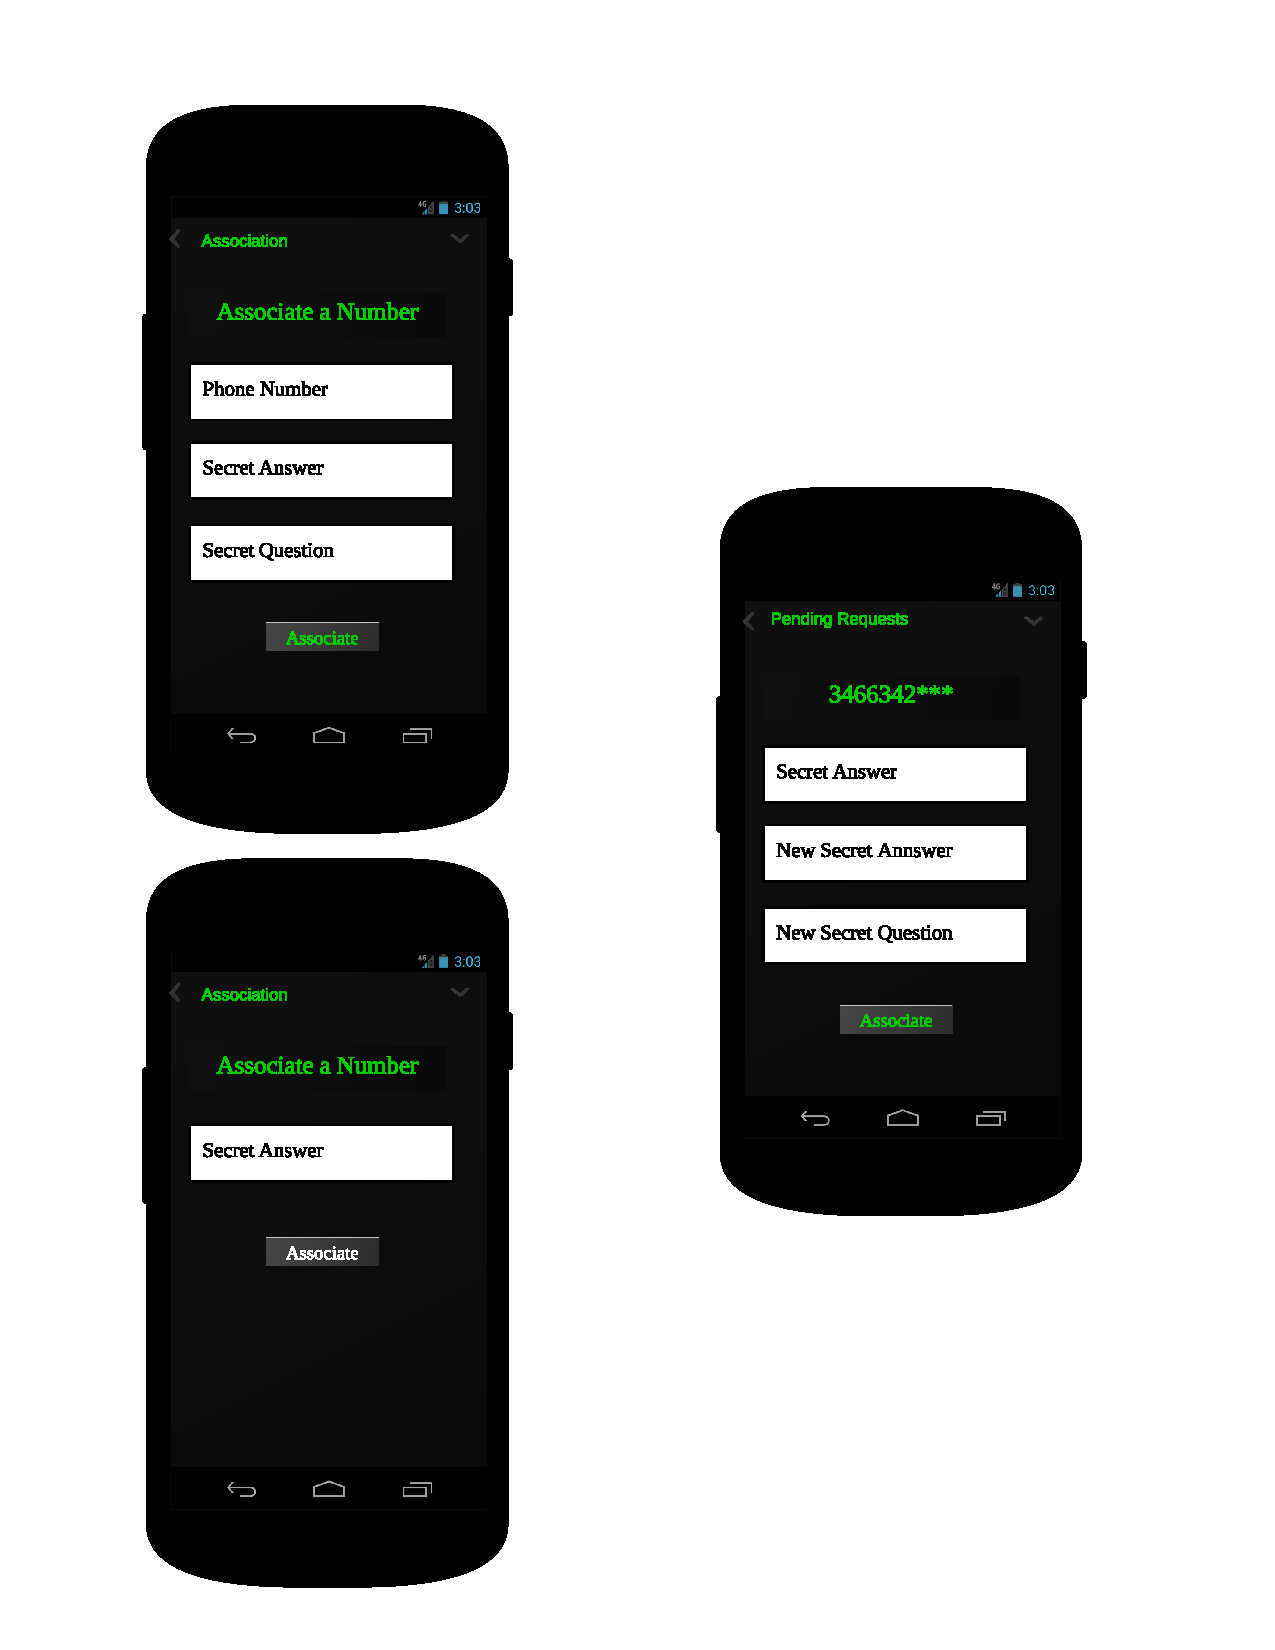
\includegraphics[scale=0.7]{images/SMP_design}

\section{Password Change}

The user types the old password, the new password and the confirmation new
password; the system checks whether the old one is correct and the new ones
are coherent and rules compliant (see initialization wizard use case). If not
an error message is prompted and nothing is done, otherwise the password is
succesfully updated and the user notified back.

\subsection{Activity Diagram}

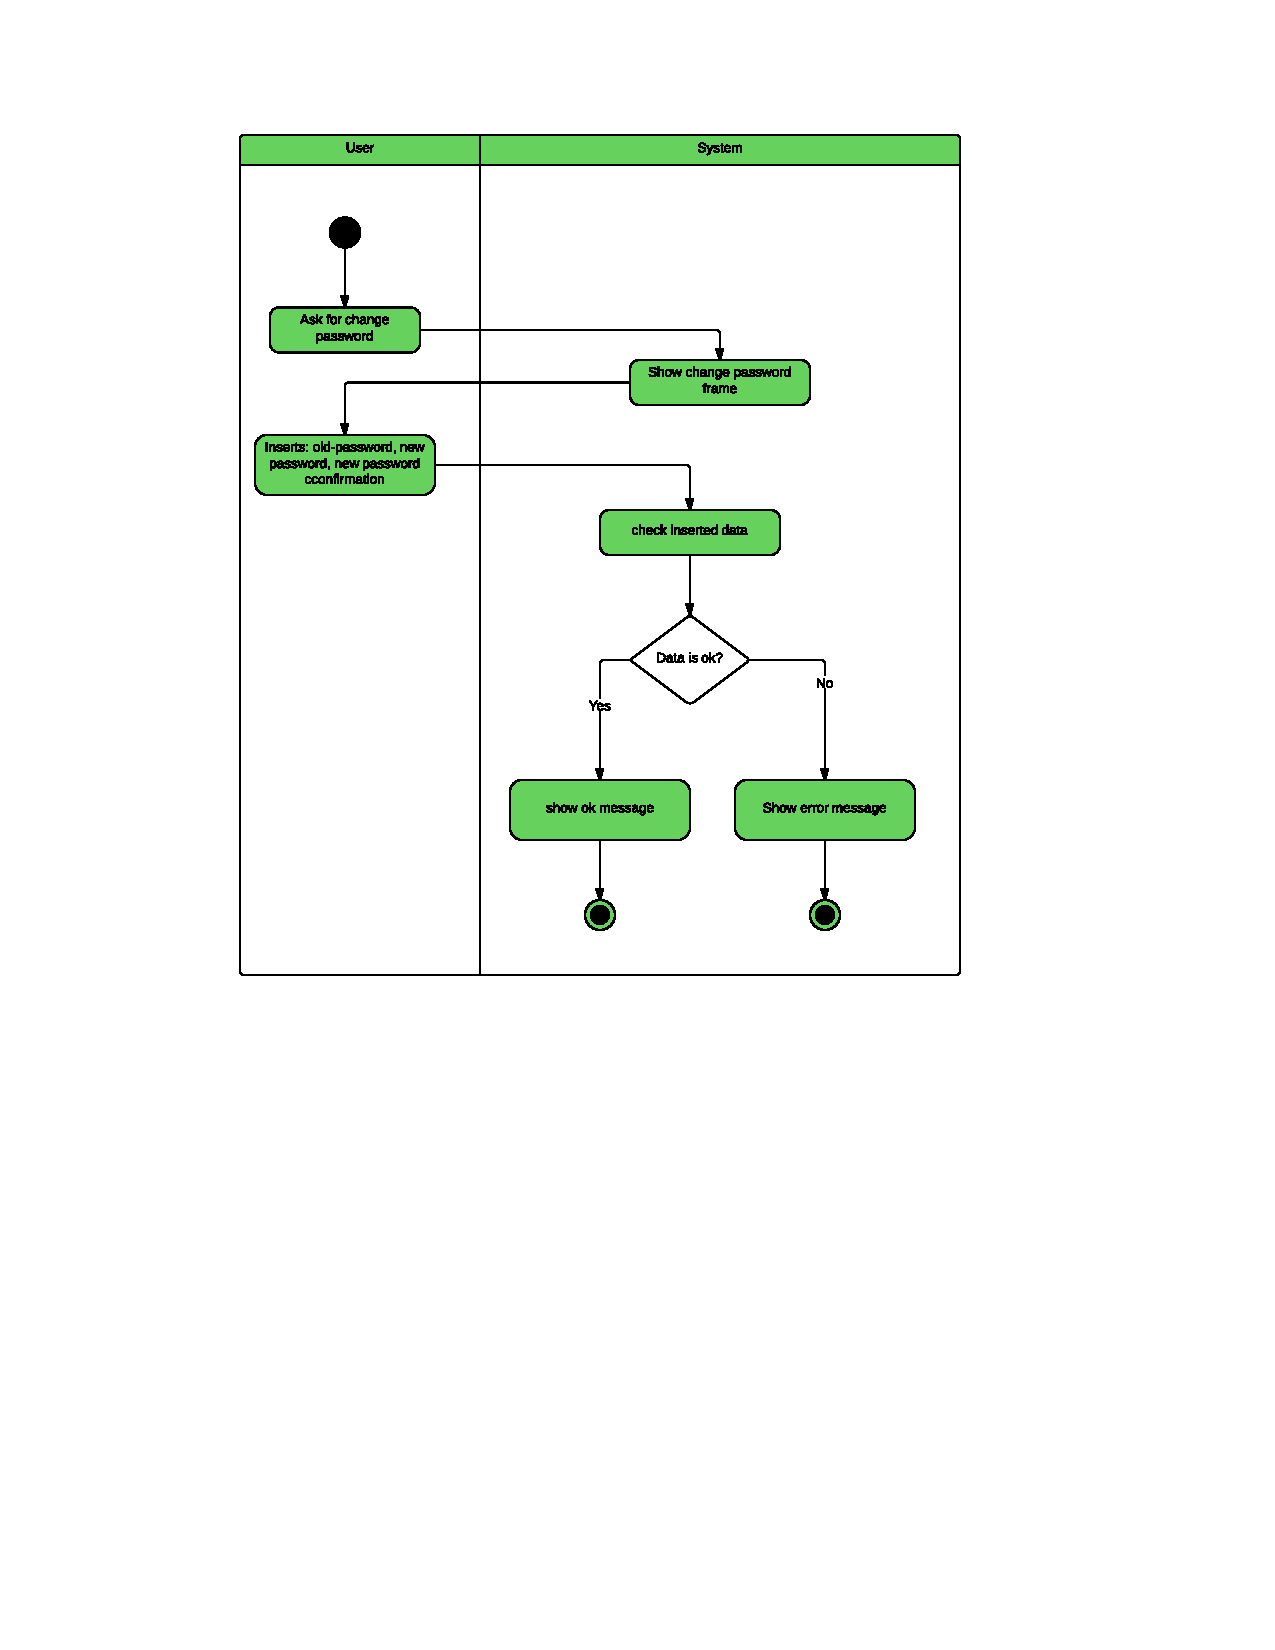
\includegraphics[scale=0.6]{images/ChangePassword_activity}

\newpage
\subsection{User Interface Design}

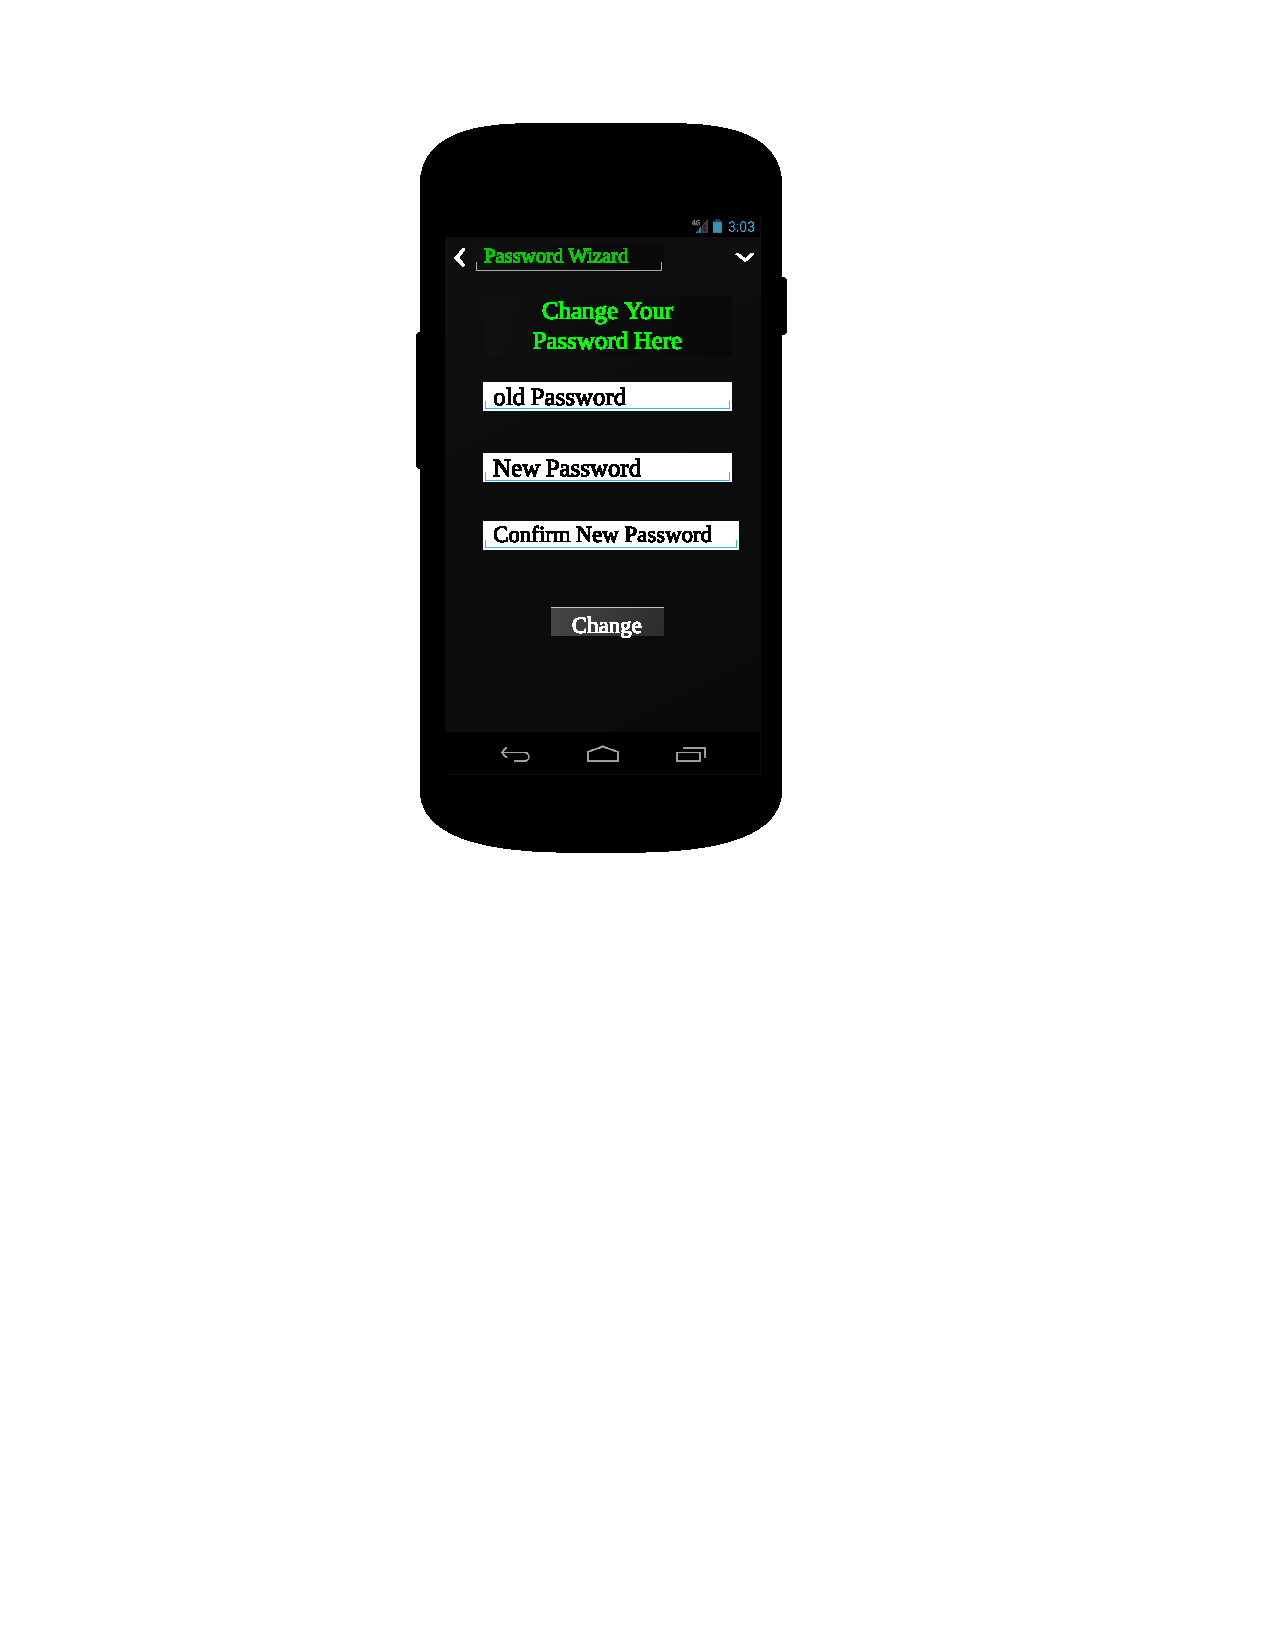
\includegraphics[scale=0.7]{images/PasswordChange_UI}

\section{Unilateral Deassociation}

The user selects from the list of his contacts the one he wants to deassociate
with and confirms his intention by clicking on the apposite button. The
relative preferences are deleted, but the "target" is not notified.


\newpage
\subsection{Activity Diagram}

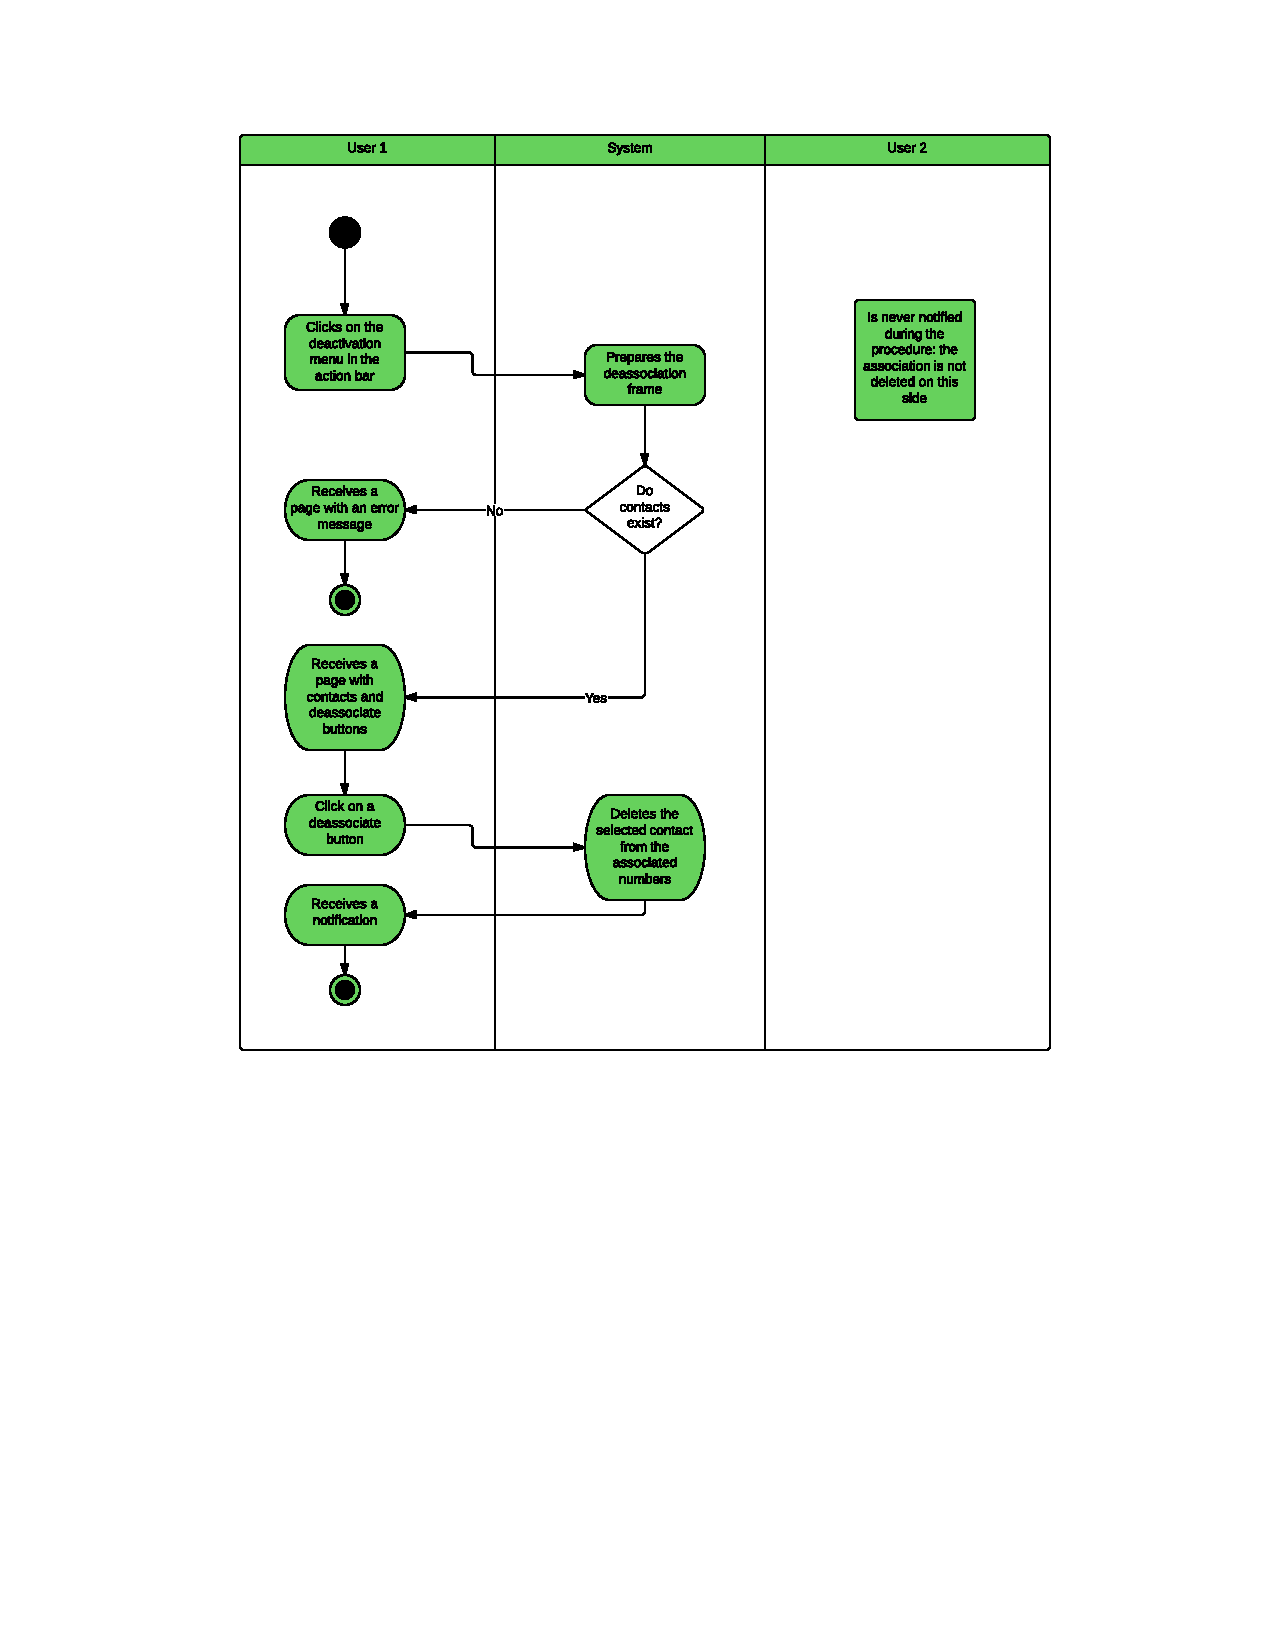
\includegraphics[scale=0.7]{images/UnilateralDeassociation}

\newpage
\subsection{User Interface Design}

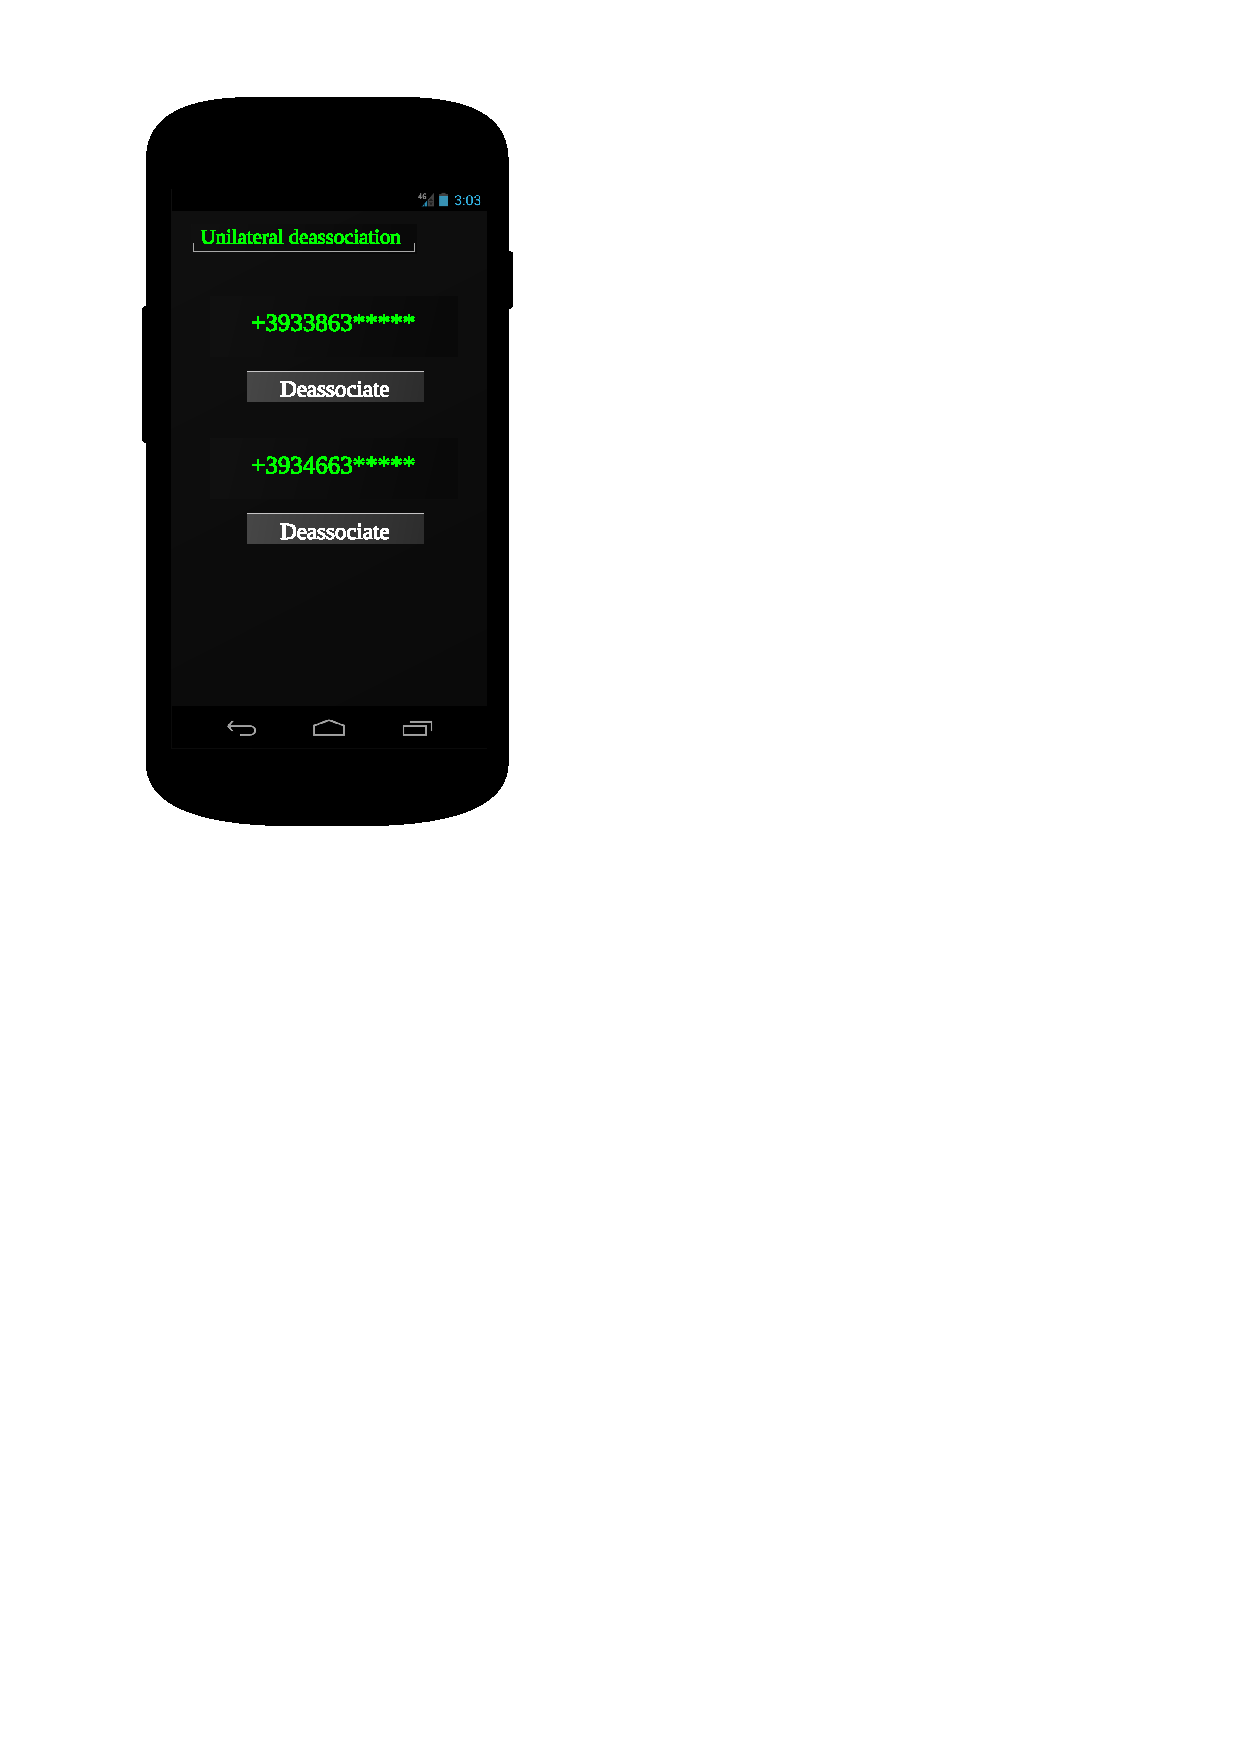
\includegraphics[scale=0.7]{images/DeassociationAndroid}

\section{Remote Localization}

The user (which sees a list of his contacts/associated numbers) types the
target password and confirms the intention to send a localize command by
clicking on the apposite button. After an handshake (done by sms exchanging)
the target phone executes the command and sends back a failure message or
his actual coordinates. The original sender receives a notification with a map
and a marker indicating the target position.


\newpage
\subsection{Activity Diagram}

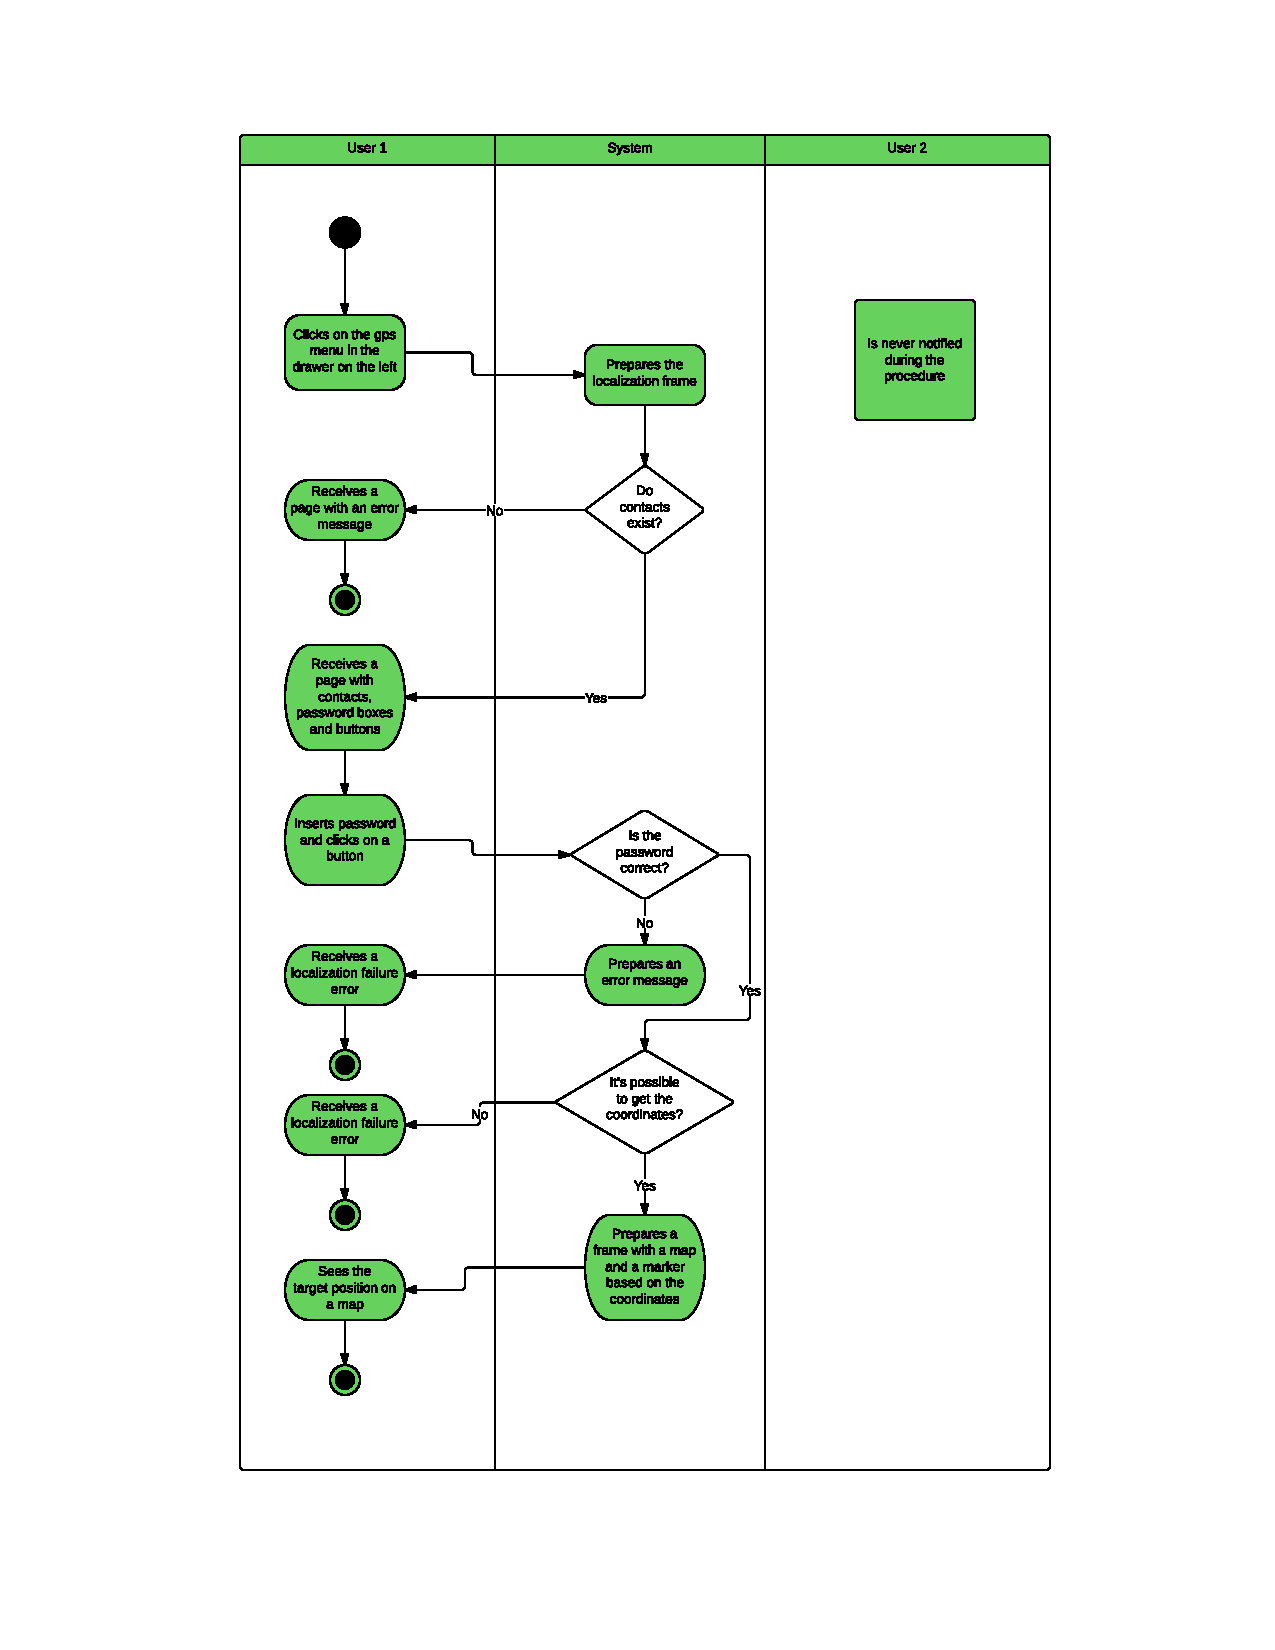
\includegraphics[scale=0.7]{images/Localization}

\newpage
\subsection{User Interface Design}

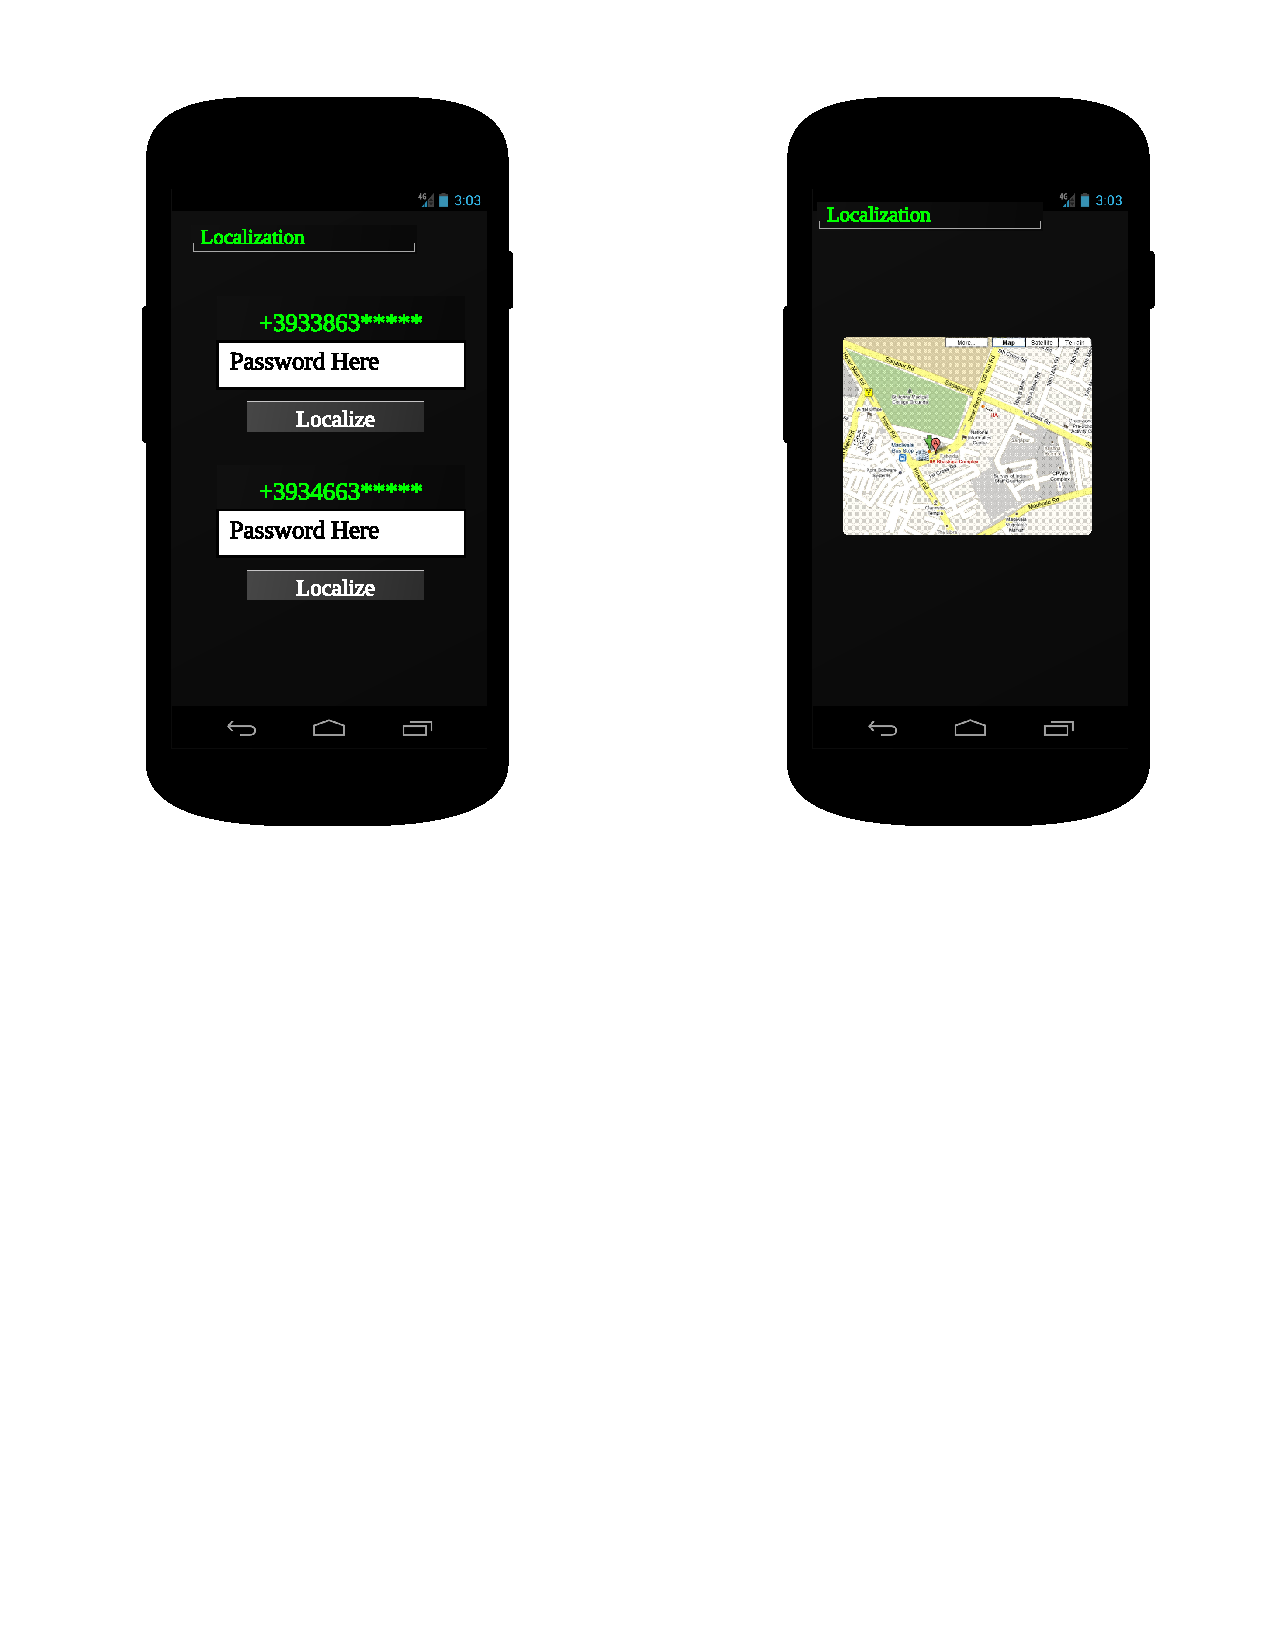
\includegraphics[scale=0.7]{images/Localization_mobile}

\section{Mobile Phone Mark}
The mark features have been left unimplemented: they are in the TODO list,
so no use cases for now.


\newpage
%\subsection{Activity Diagram}

%\newpage
%\subsection{User Interface Design}

\section{Remote Alarm Triggering: Activate and Deactivate Siren}

The user selects from his contacts the target and confirms by clicking on a
specific button the will to send a siren on/siren off command. The command
session is similar to the localization one: the only difference is that the re-
turned message is only an ack or a failure code. The siren off is simply ignored
if the alarm in not active. There is also a feature which allows a user to turn
off locally a siren by inserting the password and clicking on the button.

\newpage
\subsection{Activity Diagram}

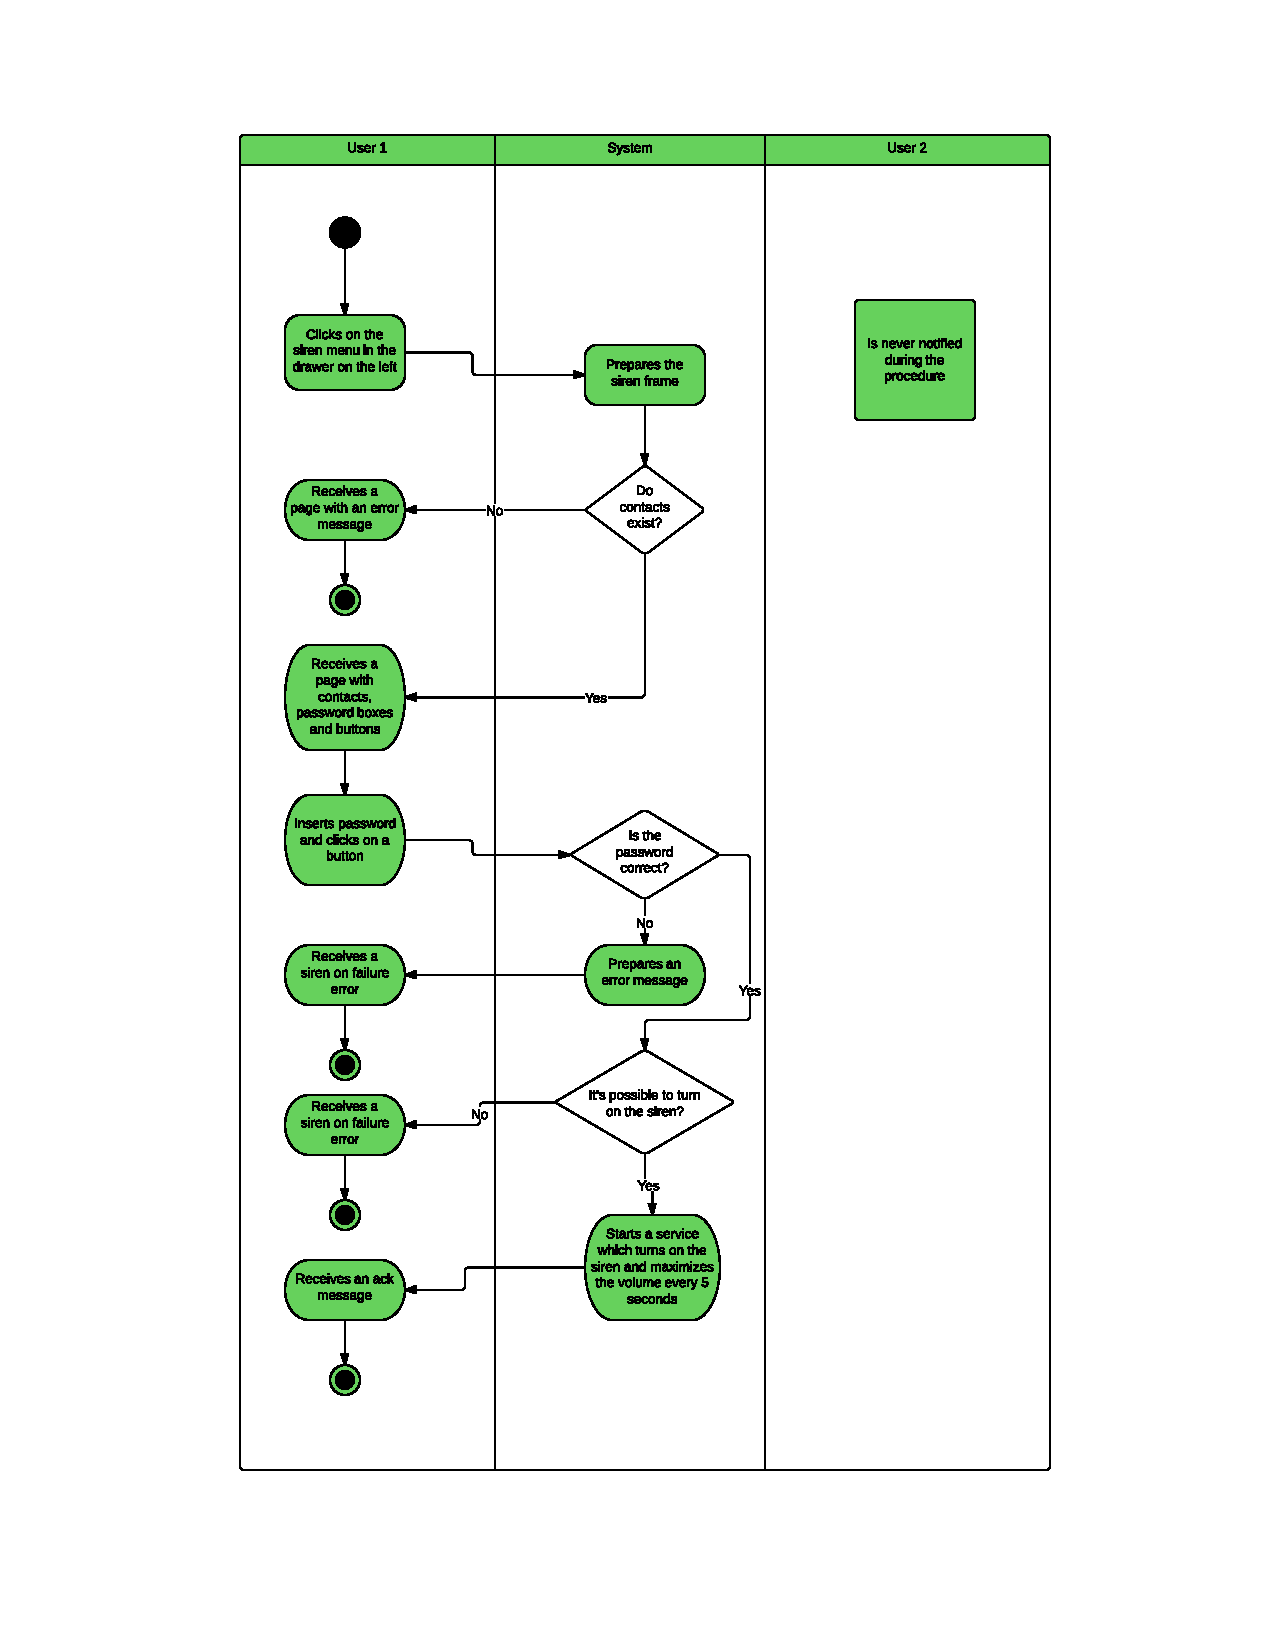
\includegraphics[scale=0.7]{images/SirenOn}
\newpage
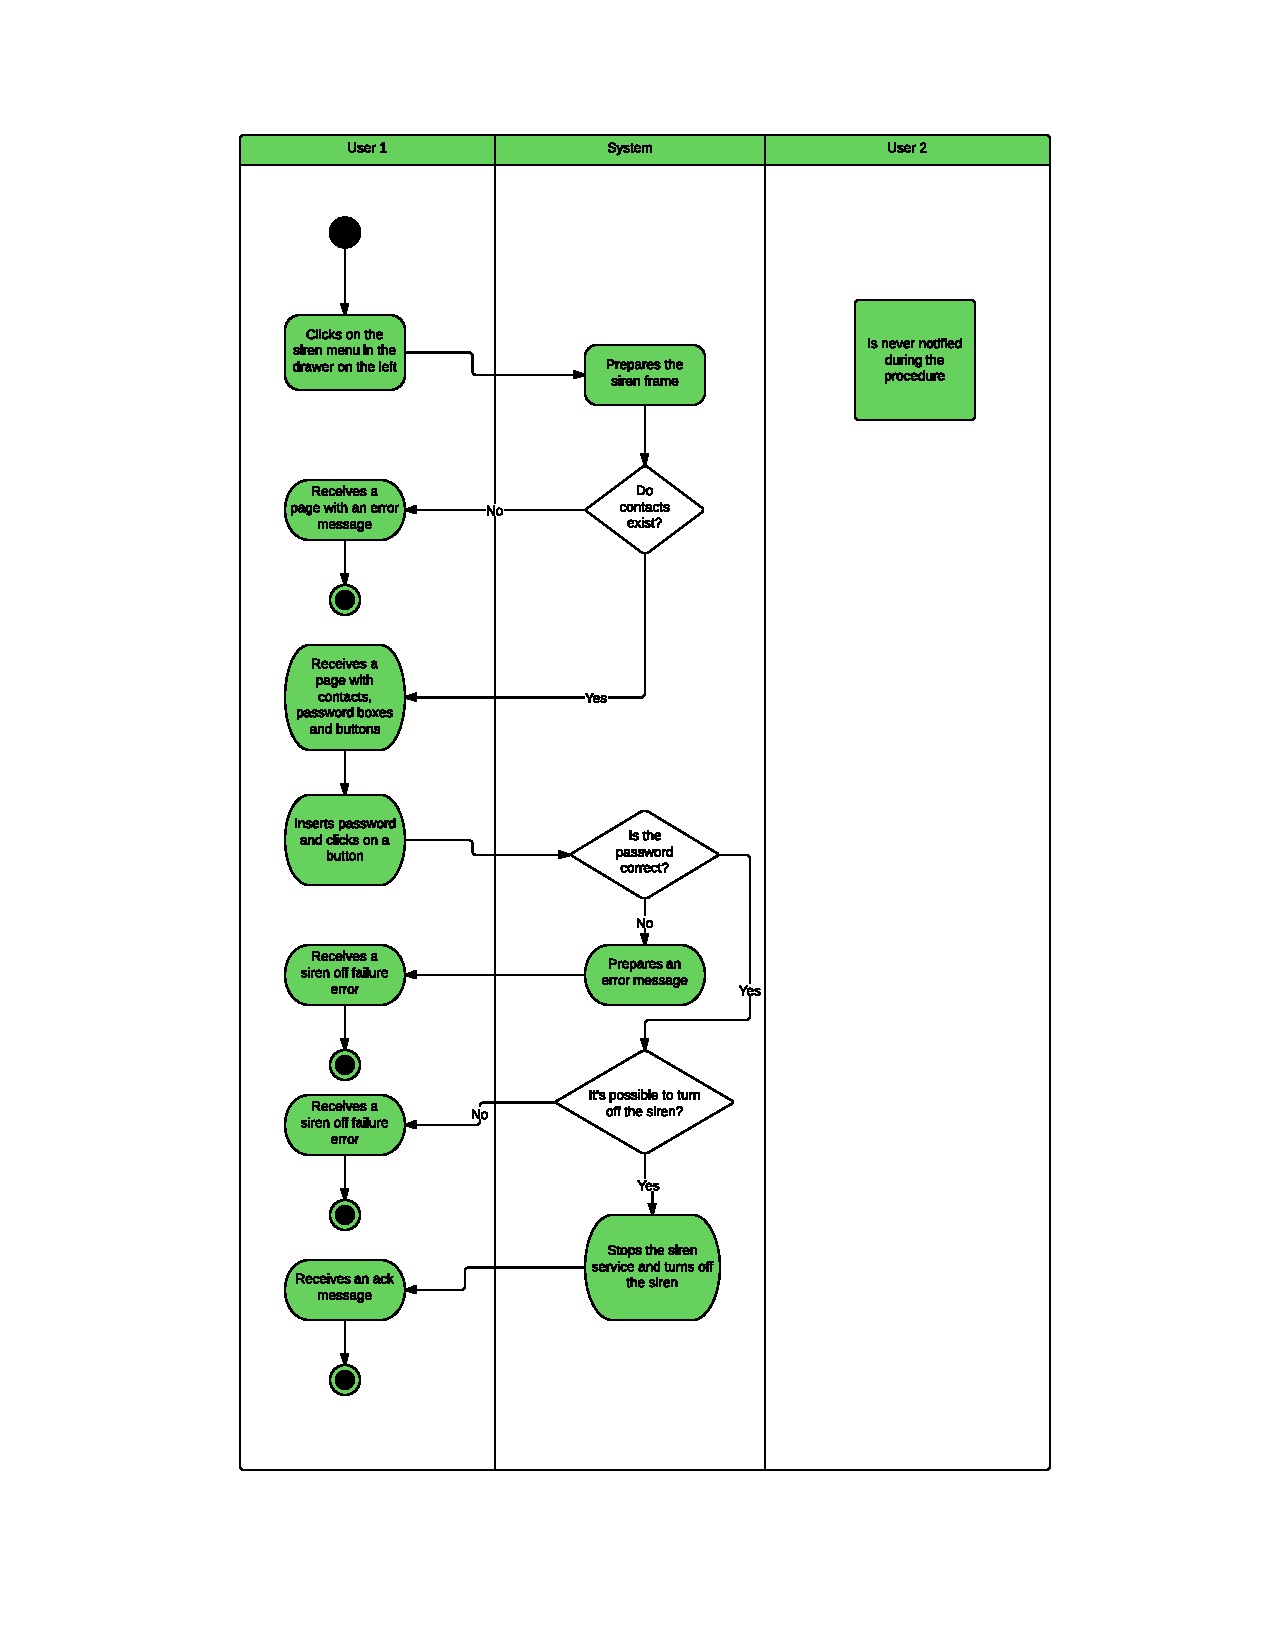
\includegraphics[scale=0.7]{images/SirenOff}
\newpage
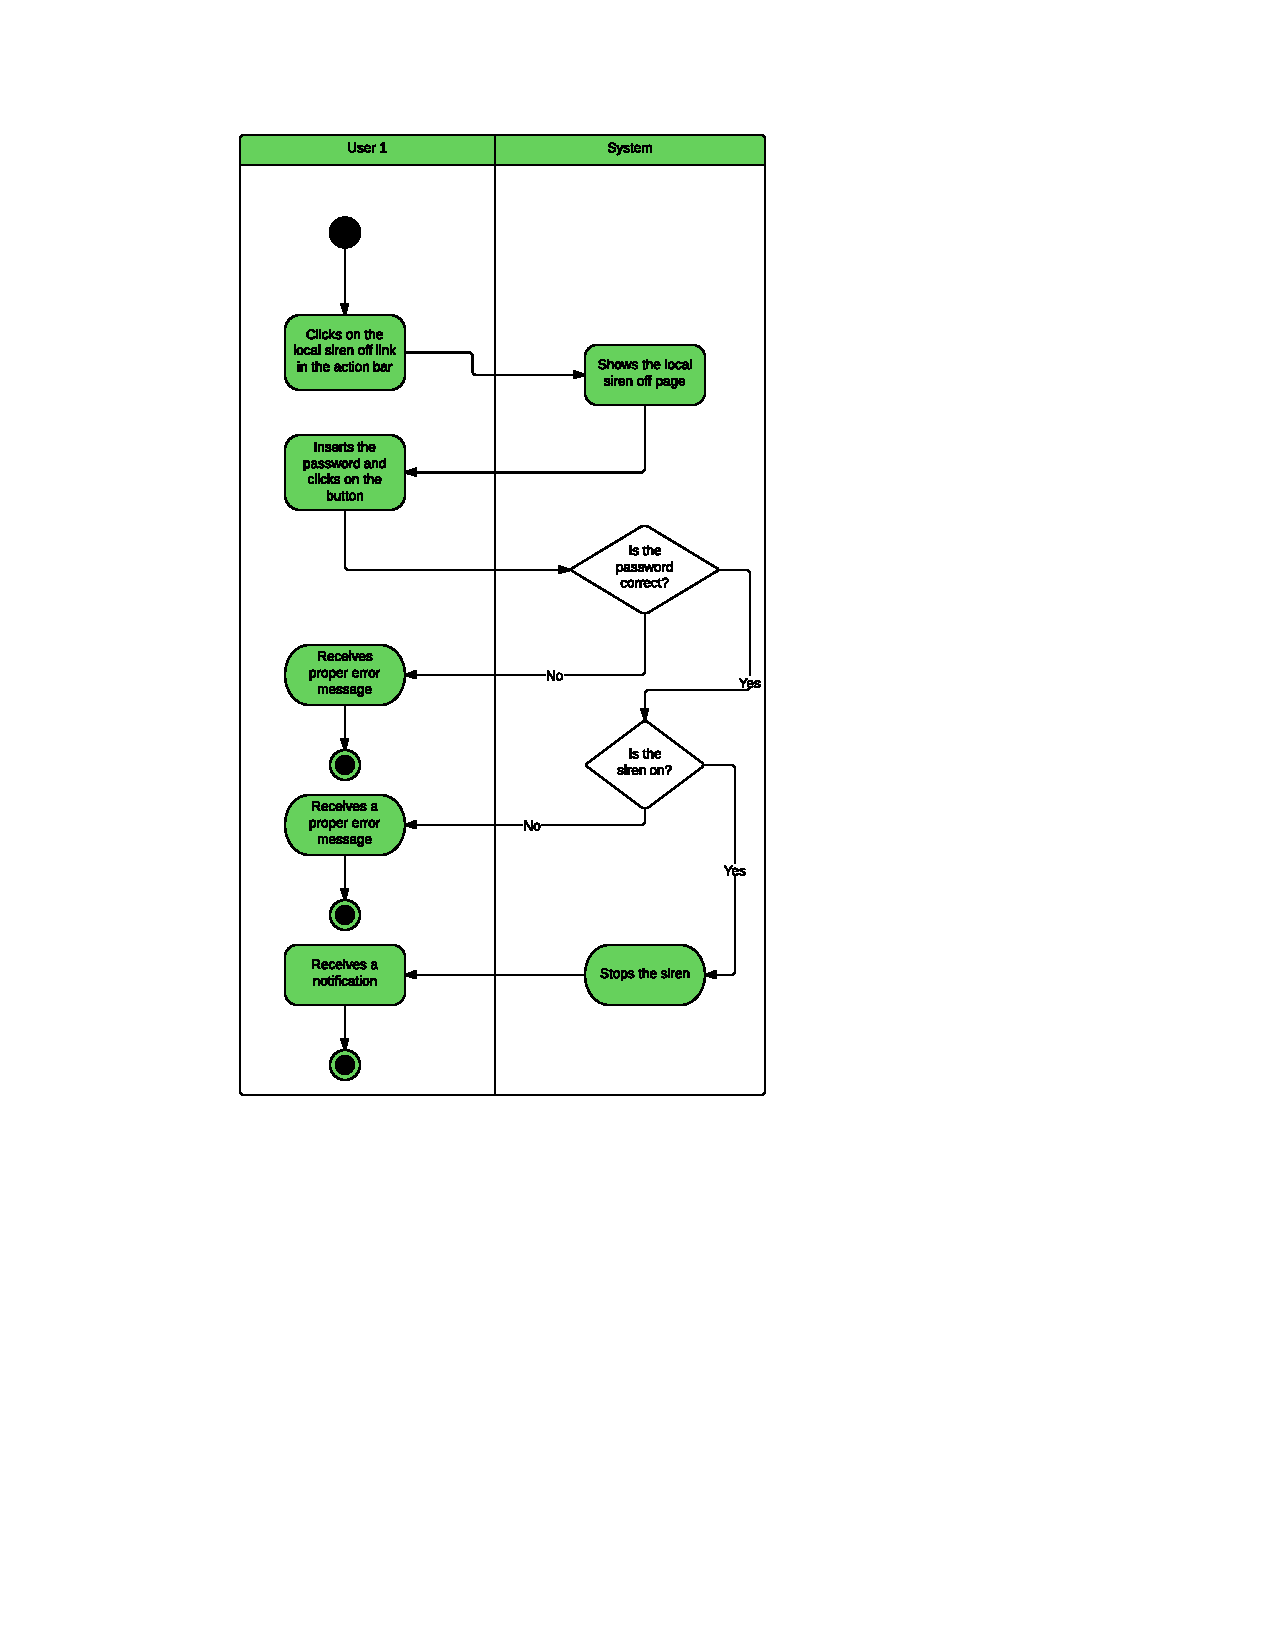
\includegraphics[scale=0.7]{images/localsirenoff}

\newpage
\subsection{User Interface Design}

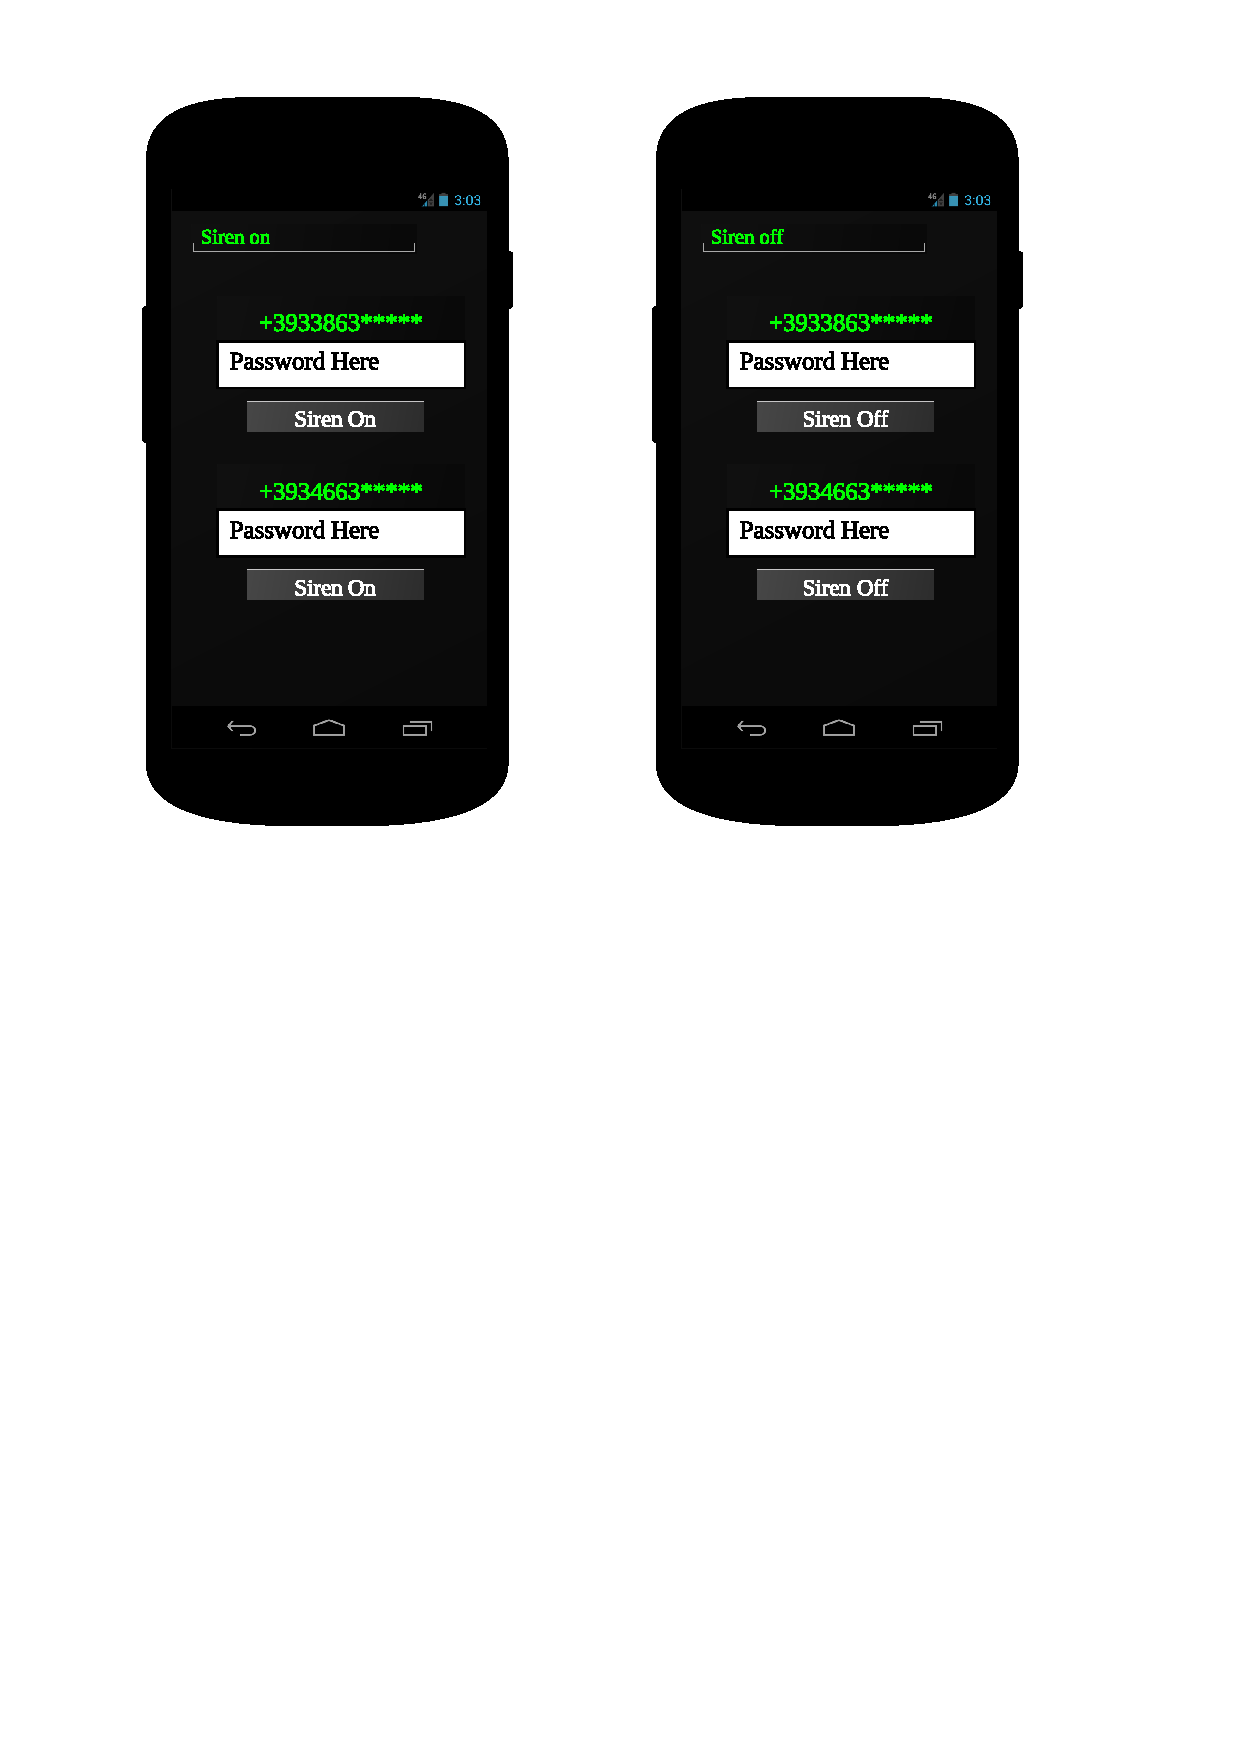
\includegraphics[scale=0.7]{images/sirenonoff_mobile}


\section{Perimeter Selection}

The perimeter selection feature, when activated, must select a circle area
centered where the cellphone is at that moment, and trigger an alarm if the
mobile phone exits from there. The circular limit has also to be visible on a
map on the telephone.


\newpage
\subsection{Activity Diagram}

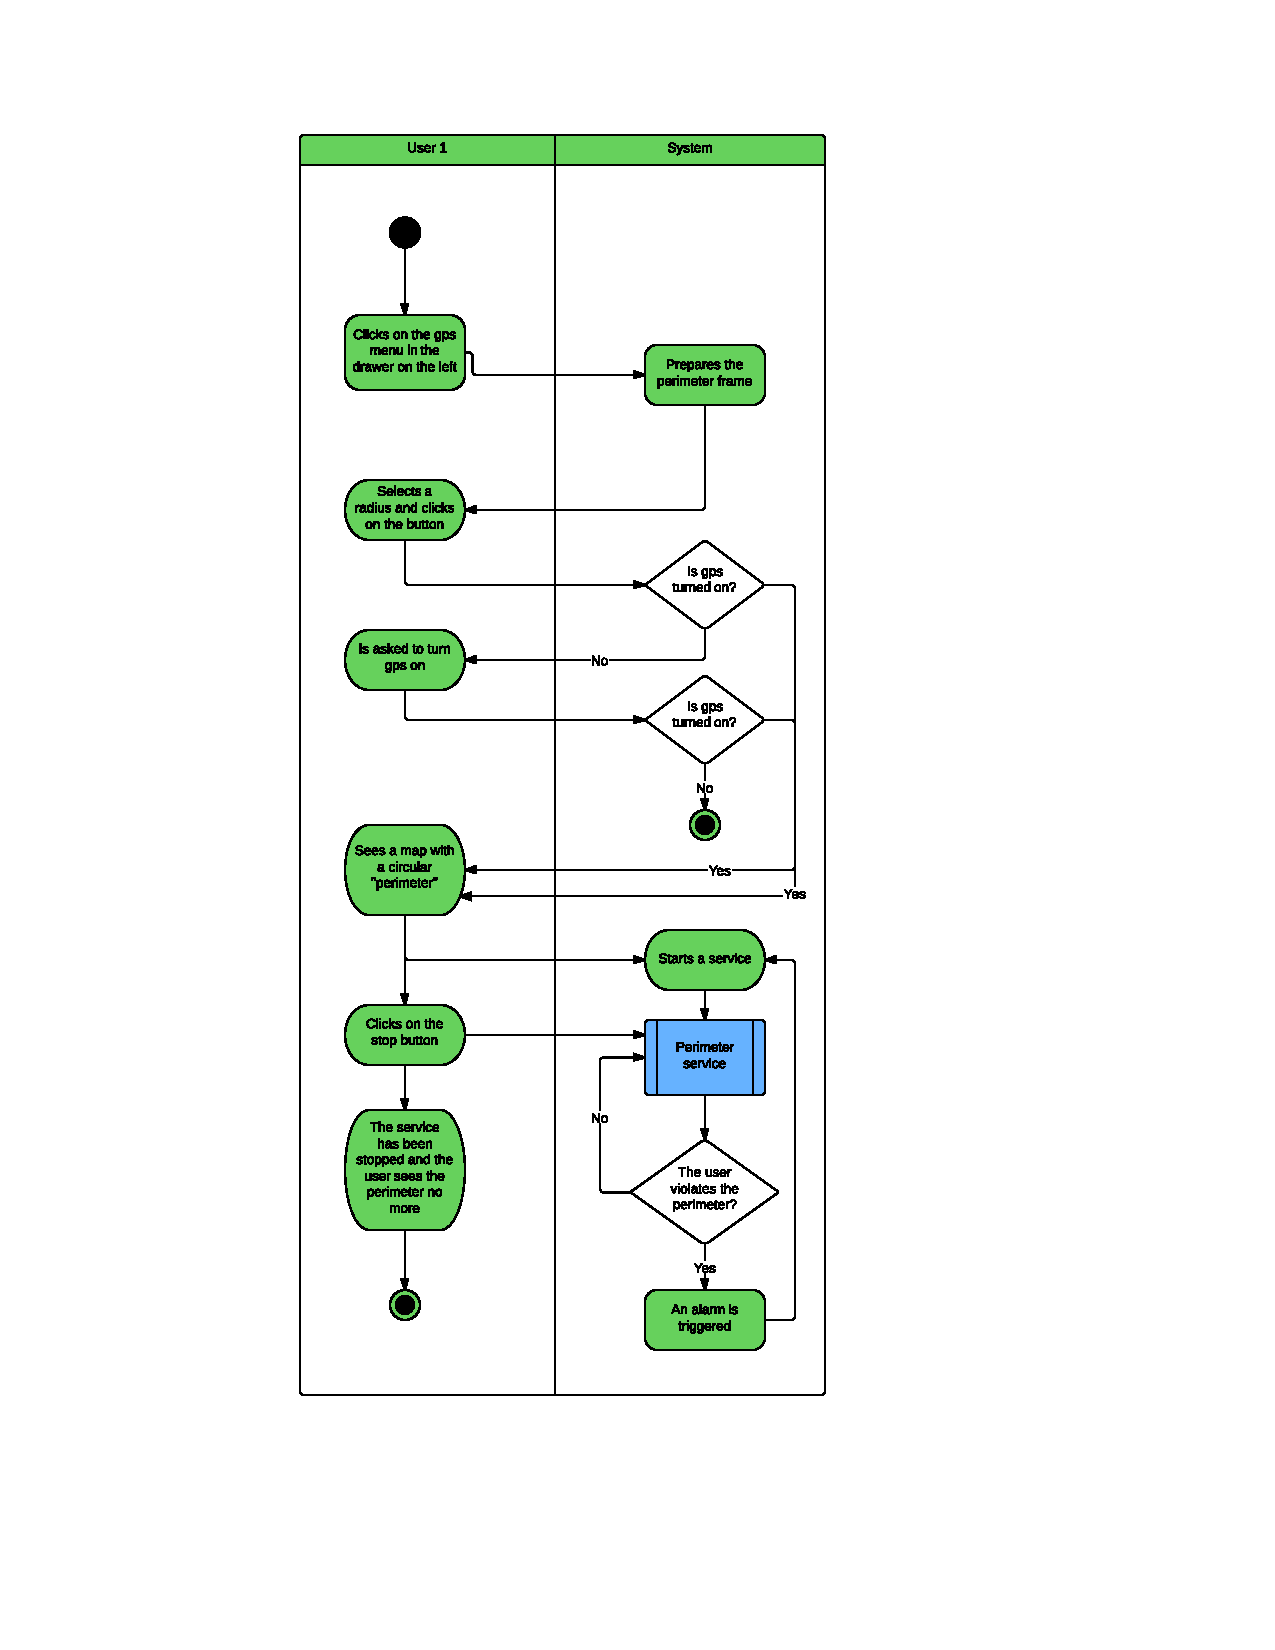
\includegraphics[scale=0.7]{images/Perimeter}

\newpage
\subsection{User Interface Design}

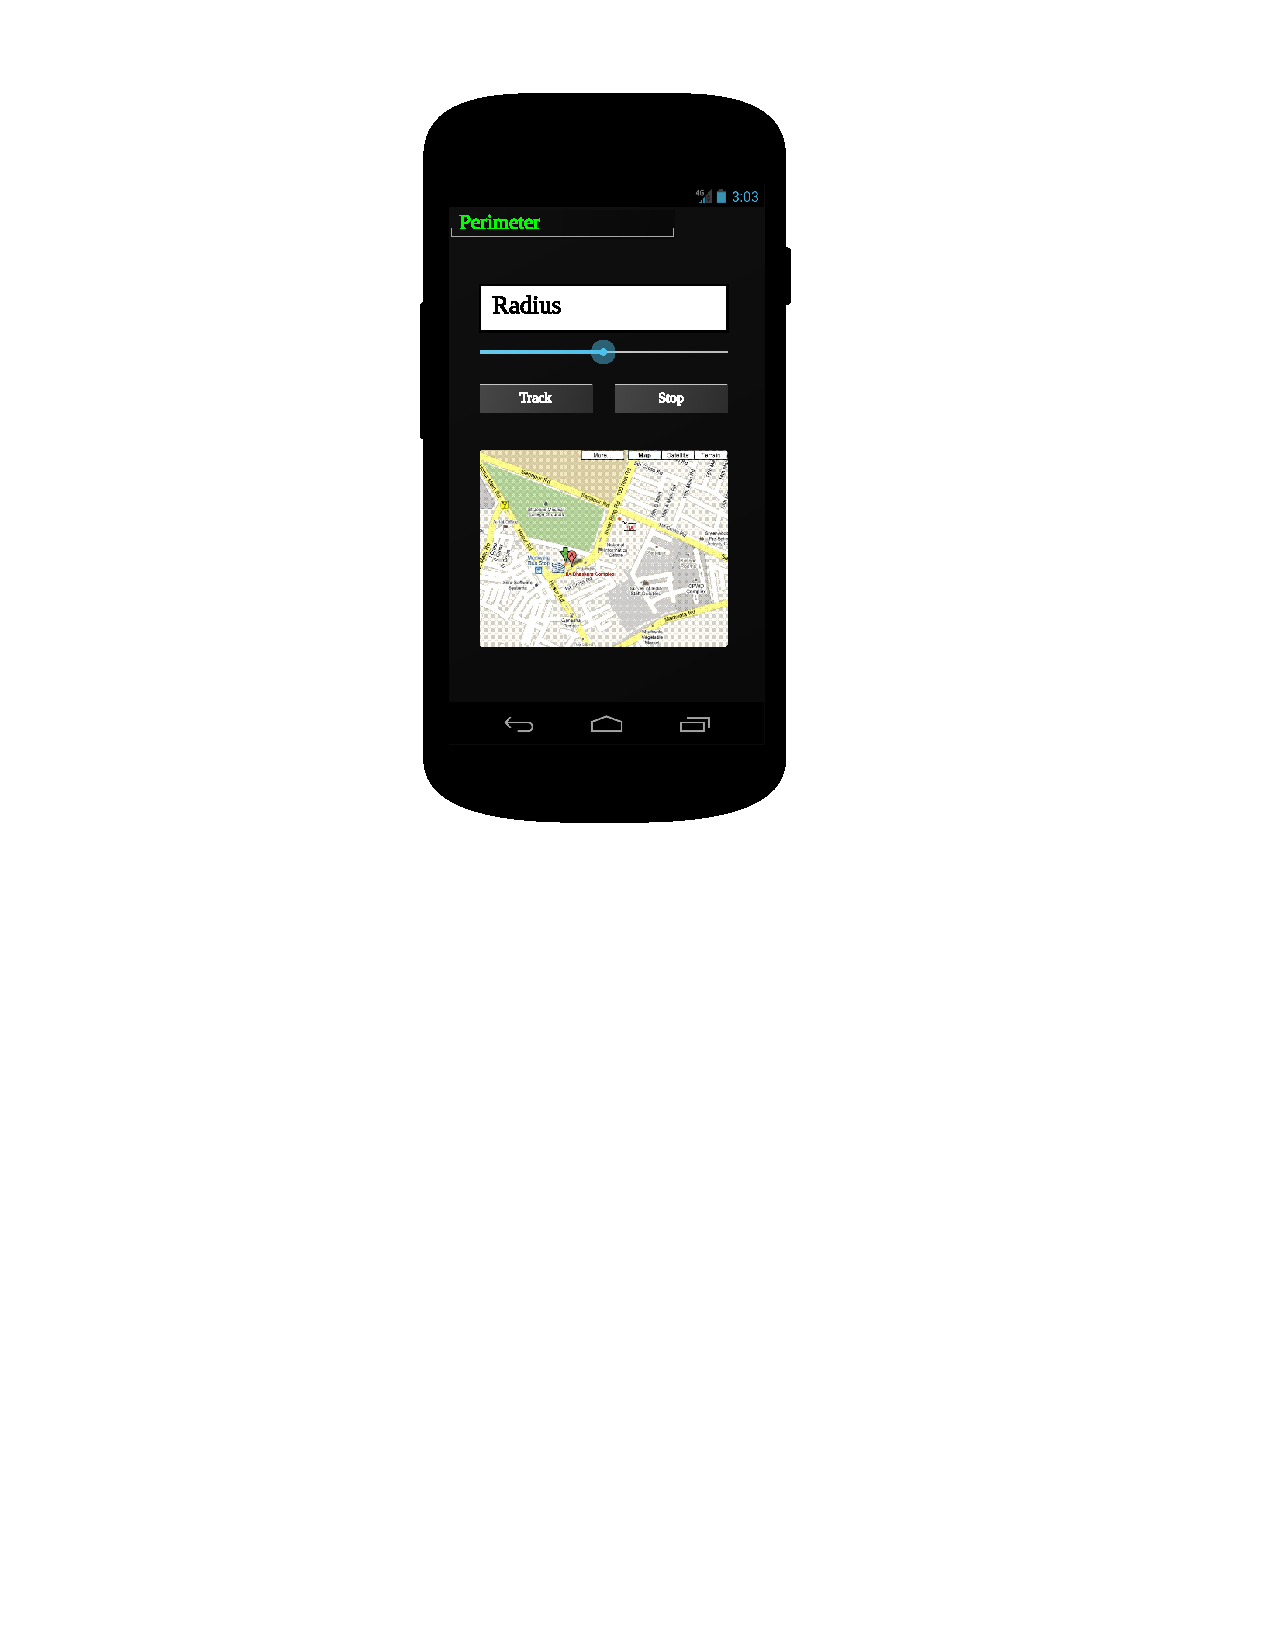
\includegraphics[scale=0.7]{images/Perimeter_mobile}

\noindent	
\Huge{\section{Design}}
%\include{contents/StateDynamicsViewpoint}
%\include{contents/InteractionViewpoint}
\subsection{Cryptography}
\small{The cryptography algorithms have been tested (with unity tests on a separate test project) on prototypes of the SMP/command messages and the results showed they were correctly implemented by Spongycastle and correctly used by us.}
\subsubsection{Elliptic Curves key pair generation}
The public/private key pair generation is done by using elliptic curves for performance and memory complexity reasons (at a fixed security level the EC keys are more than 10 times shorter compared to the RSA/DSA/ElGamal ones): a message in Android has a maximum length of 140 characters (bytes), so we had no choice if we didn't (and we didn't since it would have screwed up our crypto layer) want to use multipart messages. The curve used is a NIST standard: "secp256r1", also known as "prime256v1", which generates 256 bits long keys (we actually thought to use "secp521r1" for enhanced security, but the keys were too long). Using a named curve which is also a standard has a few advantages: first, it generates automatically all the parameters needed, second, its security has been widely tested by the cryptanalists of all the world. The generated keys are encoded into byte arrays in different ways: the private ones using the "PKCS8 encoded key specifiers", the public ones with the "X509 encoded key specifiers". It's always possible with a key factory to decode both encodings leading to keys identical to the pre-encoding ones. The keys are generated this way: given the order of the EC group and a randomly chosen point of the curve (different from the one at infinity), which is also a generator of the group, the private key is that point and the public key is computed as [priv]P, where the multiplication denoted by [integer]Point is reduced to a sequence of application of doubling a point and addition between two points. The pictures below shows graphically how these operations are defined for elliptic curves.\\

\vspace{1cm}
\begin{center}
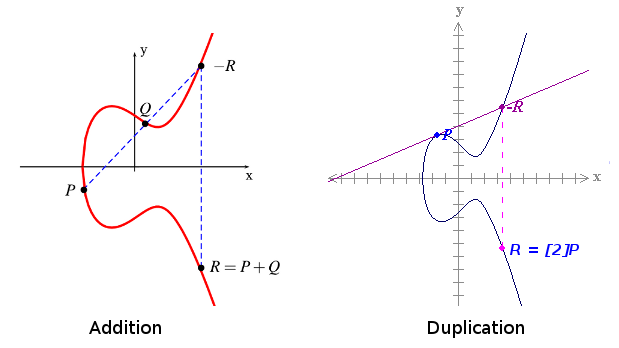
\includegraphics[scale=0.7]{images/ec}\\

\vspace{1cm}
Picture 1: ECDH schema\\
\end{center}
\section{Elliptic Curves Diffie Hellman key exchange}
The Diffie-Hellman key exchange (DH) is a key-agreement protocol used to generate a common secret between the two parts over an insecure channel; the computed secret is guaranteed to be the same for both and it's in the form of a byte array (in our case with length 32). From that secret then a deterministic key generation algorithm is able to extract a symmetric key usable for encryption/decryption. The Elliptic Curves DH (ECDH) works like this: every part computes a key pair over the same EC (we use the ones computed in the wizard), then both send their own public key to the other; now they multiply (for a proper definition on multiplication in a EC field) the public key of the other by their own private key: the result is the same due to the public/private EC keys mathematical properties as shown in the picture below.\\

\vspace{1cm}
\begin{center}
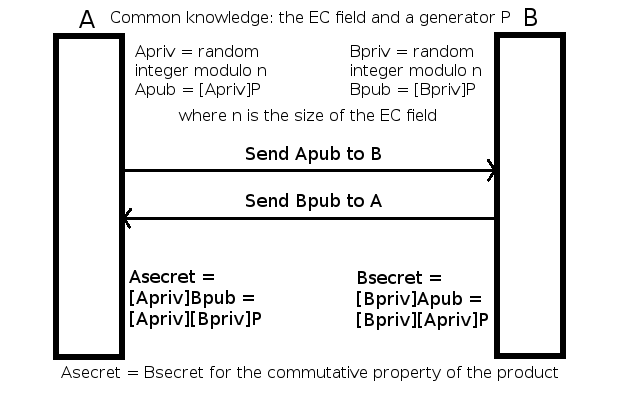
\includegraphics[scale=0.5]{images/ecdh}\\

\vspace{1cm}
ECDH schema\\
\end{center}

\vspace{1cm}
The problem with ECDH is the lack of authentication of the received public key: an active MITM could impersonate user A with user B and user B with user A by tricking them into believe his public key belongs to the other side while actually it's not true. This single point of failure is solved by embedding ECDH into SMP (see section 4.3.6).
\clearpage
\subsubsection{Elliptic Curves Digital Signature Algorithm}
Nowadays ECDSA is the best known algorithm for computing digital signature with a reasonable size, high performances and very high security: it's the EC variant of the DSS-DSA algorithm and it works like this: assumed the signer (sender) has a keypair based on EC (Apriv = s, Apub = [s]P), and the receiver knows Apub and trusts it, and both parts know the curve and its parameters (n = size of the group, P a generator of the group), then:
\linebreak
\begin{enumerate}
\item The signer chooses a random integer $r$ $mod$ $n$ such that $n > 0$ and $GCD(r,n) = 1$
\item The signer computes $[r]P = (x,y)$
\item If $x = 0$ goto step 1, else the signer stores $x$ as $k$
\item The signer computes $r^{-1}$ $mod$ $n$ and $e = SHA-1(m)$ where $m$ is the message to sign
\item The signer computes $z = r^{-1}(e + sk)$ $mod$ $n$
\item If $z = 0$ goto step 1, else the signature is made by $(k,z)$
\linebreak
\end{enumerate}
Verification:
\linebreak
\begin{enumerate}
\item The receiver checks whether $k$ and $z$ are $mod$ $n$ and positive not null integers, if not, the signature is not valid
\item The receiver computes $e = SHA-1(m)$ and $w = z^{-1}$ $mod$ $n$
\item The receiver computes $u_{1} = ew$ $mod$ $n$ and $u_{2} = kw$ $mod$ $n$
\item The receiver computes a point $X = [u_{1}]P + [u_{2}][s]P$ and stores it as $(x,y)$
\item If $X$ is the point at infinity or is not verified $x = k$ $mod$ $n$, the signature is not valid, otherwise is valid.
\end{enumerate}
\subsubsection{PBKDF2 with HMAC-SHA-256}
The Password Based Key Derivation Function \#2 is a deterministic key-derivation algorithm which generates a symmetric crypto key with a desired length by taking in input a password or a passphrase (in our case the secret from ECDH) and a salt (which makes possible to derivate different keys from the same password) and doing a certain number (4096 in our case) of application of a pseudorandom function (HMAC-SHA-256 in our case) to them in the so called "key stretching", which makes very hard the use of rainbow tables for cryptanalysis.
\subsubsection{AES-256-GCM}
\small{The Advanced Encryption Standard is the symmetric encryption standard algorithm (NIST FIPS-197) almost worldwide since 2001, and it's known for high performances and security against cryptanalysis; in the application we employed its version with a 256 bits key, which has a security margin comparable to RSA with a 15360 bits key. Actually, since it's used in Galois/Counter Mode (GCM), it does not encrypt directly the plaintext, but it's instead used together with a 12 bytes initialization vector IV (which doesn't need to be secret, but unpredictable for every encryption, so the best choice is to pick it up randomly) to generate a pseudorandom keystream, which is then XORed to the plaintext: basically the block cipher simulates a stream cipher (so no padding is needed for the plaintext, whose length, thus, does not need to be a multiple of 16 bytes, like in direct encryption, which is a good thing, considering the 140 bytes limit for Android messages) which simulates a One Time Pad (OTP), the only cipher perfectly secure. Obviously AES-GCM is not perfectly secure because, frist, soon or later, a new key will be equal to one used in the past (not so soon though), second, the key is shorter than the plaintext and, third, the keystream is only pseudorandom. In addition to this the GCM mode generates also a 16 bytes Message Authentication Code (MAC) which is prepended to the ciphertext in order to provide an additional integrity check. Before the decryption (which needs of course the same IV and the same key) the message integrity is verified and, if it's not the case, an exception is raised and the command session is aborted. In GCM mode it's also possible to attach to the ciphertext some non-encrypted data (called Additional Authenticated Data, AAD) which are used along with the ciphertext itself to produce the MAC; in our case this feature is useless, so no AAD.\\The three pictures below show the encryption and the decryption under GMC (P = plaintext, K = key, C = ciphertext, A = AAD, T = MAC) and the AES encryption/decryption used to generate the keystream.}\\

\vspace{1cm}
\begin{center}
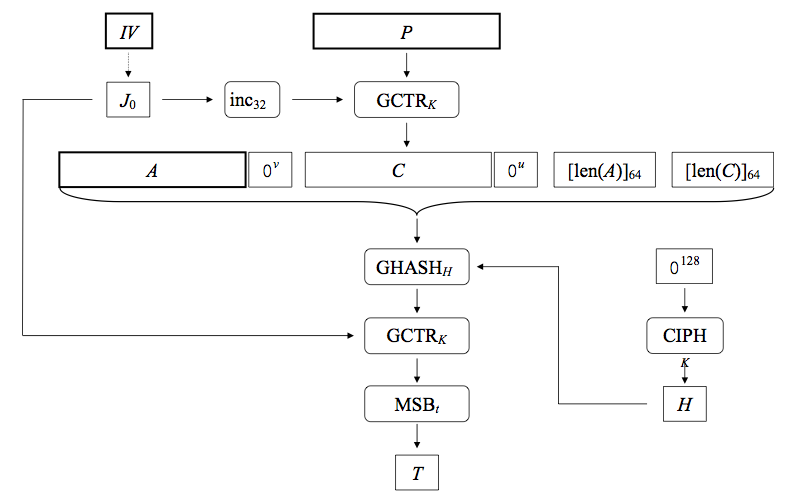
\includegraphics[scale=0.5]{images/aesgcmenc}\\

\vspace{1cm}
Picture 1: Encryption in GCM mode of operation\\
\clearpage
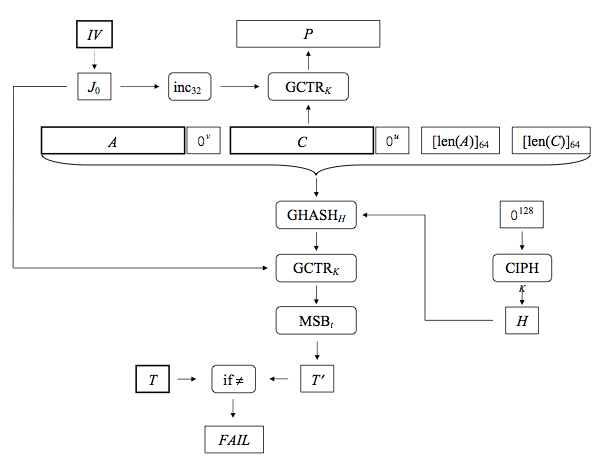
\includegraphics[scale=0.6]{images/aesgcmdec}\\

\vspace{0.5cm}
Picture 2: Decryption in GCM mode of operation\\

\vspace{2cm}
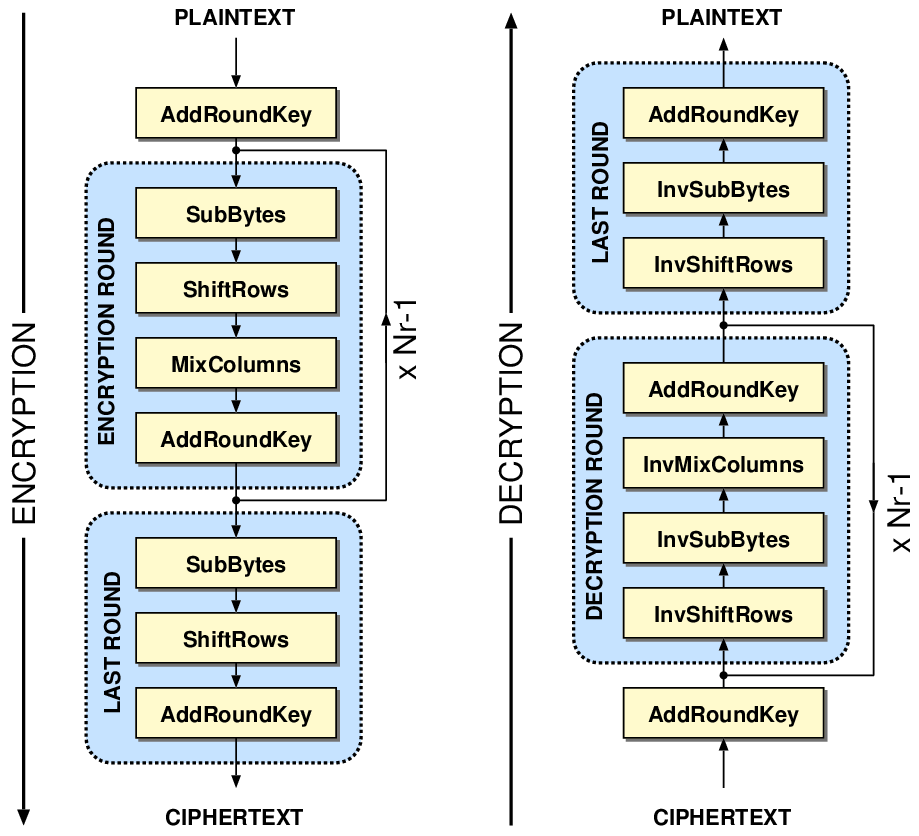
\includegraphics[scale=0.3]{images/aes}

\vspace{0.5cm}
Picture 3: Encryption/Decryption in AES\\
\end{center}
\clearpage
\subsubsection{Socialist Millionaire Protocol}
The Socialist Millionaire Protocol purpose is to mutual authenticate public keys, so that a logical binding is created between a key and a phisical device; this solves the active MITM problem. Since a java implementation of the original SMP was not available, we coded our own version of it, which also embeds ECDH to spare time: the whole protocol is based on messages exchanging.
\paragraph{Public key request} \hspace{0pt} \\
When someone wants to associate his telephone with another one (and vice versa, which is automatic) and confirms his will by clicking on the apposite button, the system stores the inserted secret question and its answer, then generates a message made by the header "CODE1FFF" (intended hexadecimal as all the similar codes later descripted) and a null body and sends it to the other mobile, writing into the preferences that the message has been sent. The meaning of the code is a request for the other public key. The receiver, after verifying (in the so called from now on "message validation") the message arrived in a right moment (i.e.: not during another SMP session with the same user), writes into the preferences the occurred event.
\paragraph{Public key sending} \hspace{0pt} \\
The response to a public key request is a message made by the header "CODE2FFF" and the public key itself; of course also the happening of this sending is saved in the preferences updating the SMP log file. The receiver, after the sms validation, writes into the preferences the event and stores in the so called "KeySquare", a keyring of the not yet validated keys, a Base64 representation of the key.
\paragraph{Question sending} \hspace{0pt} \\
After receiving the public key, the system saves the event in the preferences, then fetches from there the previously stored secret question, sends it to the other appended to the header "CODE3FFF" and saves into the preferences this sending event. The receiver validates the message, updates the SMP log file in his preferences and stores the received question.
\paragraph{Hash sending} \hspace{0pt} \\
After storing the secret question, the system notifies the user of the existence of a pending association request: the person at this point can decide to refuse (which is managed as an error) or to insert the answer to the secret question and confirm. If we are in the first half of the SMP (the user who can accept/refuse to send his key has not validated the other public key), also the secret question/answer to be used in the second half must be provided (basically they are stored in the preferences). Now the system computes a SHA-256 hash of the concatenation of the public key and the given answer; the next step is sending to the other such hash prepended by "CODE4FFF" and to update the SMP log. The receiver validates the message and updates his log too.
\paragraph{Ack and password salt sending}
\paragraph{Second half} \hspace{0pt} \\
After validating the ack message and saving the salt, the  system checks whether exists in the keysquare an entry for the other mobile public key. If yes the SMP is successfully over, otherwise a public key request message is sent and the log is updated, starting this way the second half of the SMP.
At the end of the SMP both logs are filled, both public keys are validated, and both systems computed the same 32 bytes common secret.
\paragraph{Error management} \hspace{0pt} \\
Every ecception raised by the system, every message not validated, the hashes mismatch and the user refuse to the association are all treated in the same way: all the preferences relative to the other user are deleted, then a message made by "CODE6FFF" is sent to the other. Such code is accepted by the system if and only if the SMP session is still pending and not finished; the code has the effect of making the system delete all the preferences relative to the other mobile. After that a new "CODE6FFF" is sent; the whole thing doesn't loop because the "CODE6FFF" is ignored if there are no saved preferences relative to the other cellphone. This ensures in case of errors both telephones delete the preferences (and the SMP log) in which is present a reference to the other one, so in an eventual next SMP between the same two mobiles there won't be errors due to already existent preferences.
\subsubsection{Command Protocol}
\paragraph{First message}
\paragraph{Second message}
\paragraph{Third message}\hspace{0pt}\\
When m2 is received before the timeout (if not it will be treated as m1, and obviously will be rejected in the header validation phase), the timeout is stopped, the signature/header validations are done, the iv is stored and the decryption key for m4 computed and saved in the preferences. Now m3 is created in this way: AES256GCM(key-for-m3, iv-for-m3, SHA256(password) + command code + a space character separator + ecdsa signature); after that m3 is sent to the other, the log is updated and the timeout restarted.
\paragraph{Fourth message}\hspace{0pt}\\
When m3 is received within the timeout (which is immediately stopped), the decryption (which includes the MAC integrity check) is performed, followed by the signature verification. After that, various actions are performed depending on the command received and m4 is constructed as  AES256GCM(key-for-m4, iv-for-m4, header + fixed length body with padding + ecdsa signature) and sent. Finally the log is updated and the preferences of the session deleted, so that a new session can begin. When m4 is received (within the immediately stopped timeout) and passes the usual decryption/validations steps, different actions are performed depending on what was the sent command and, after everything is done, the session preferences are deleted on this side too.
\paragraph{Error management} \hspace{0pt} \\
Every ecception raised by the system, every message not validated, the hashes mismatch and the user refuse to the association are all treated in the same way: all the preferences relative to the other user are deleted, then a message made by "CODE6FFF" is sent to the other. Such code is accepted by the system if and only if the SMP session is still pending and not finished; the code has the effect of making the system delete all the preferences relative to the other mobile. After that a new "CODE6FFF" is sent; the whole thing doesn't loop because the "CODE6FFF" is ignored if there are no saved preferences relative to the other cellphone. This ensures in case of errors both telephones delete the preferences (and the SMP log) in which is present a reference to the other one, so in an eventual next SMP between the same two mobiles there won't be errors due to already existent preferences.
\paragraph{Timeout management}\hspace{0pt}\\
When a timeout countdown reaches zero, the command session log in the shared preferences is deleted, so any future command message will be treated as m1 (and discarded if it is a "late" m2 or m3 or m4).
\clearpage
\section{Open Issues and TODO list}
Our application has still some issues and some incomplete features: the next subsections speak about them.
\subsection{Unilateral Uninstallation}
If the application is removed (or the preferences deleted) on a telephone, then, after a reinstall, the owner of that mobile phone won't be able to reassociate to his old contacts, since on the other side the situation will still look like a completed association, so any SMP message coming from an already associated phone (including IDontWantToAssociate) will be simply discarded in the message validation phase. A possible workaround is to notificate to all the contacts when the application is uninstalled, but\\
\begin{itemize}
\item it may not be always possible ("dirty" uninstall ways);
\item the application is mainly intended to be used by the same person on two telephones, so the user has likely the control on both (he is likely the one to uninstall the app);
\item a validation of such message (real or fake or error) is not trivial.
\end{itemize}
\vspace{0.7cm}
The second possible solution is to create a way to locally delete some preferences relative to the other user(s).
\subsection{Association Deletion}
Our application lacks a way of deleting a specific association without uninstalling the application (see previous subsection): that's a TODO.
\section{The Mark Features}
The "mark" features (stolen, lost, both, found) are all left unimplemented (despite the application being scalable: the visitor pattern already contains the classes needed to implement them). That's also a TODO.
\clearpage
\noindent
\Huge{\chapter{Appendix C: Testing}}
\subsection{Cryptography}
\small{The cryptography algorithms have been tested (with unity tests on a separate test project) on prototypes of the SMP/command messages and the results showed they were correctly implemented by Spongycastle and correctly used by us.}
\subsection{Protocols}
\clearpage

\noindent
\Huge{\section{Installation and usage manual}}
\subsection{Installation}
\subsection{Usage}
\small{The user, after doing the initialization wizard can access the functionalities by clicking on two buttons: the one on the left upper part of the screen opens the drawer which provides access to the remote sms control (siren/localization) and to the perimeter and local siren stop features. The one on the right upper part opens the action bar (actually different telephones may have different way to open the action bar, but that's independent from our application) which provides access to the association, password change, deassociation and pending requests features.}
\clearpage
% Appendici


% --------------------------------------------------------------------------------------------------------------------
% Bibliografia - nothing for now!
%\bibliographystyle{plain}
%\input{contents/bibliography.tex}

% --------------------------------------------------------------------------------------------------------------------

\end{document}